\documentclass[../ClassicThesis.tex]{subfiles}
\begin{document}

%************************************************
\chapter{Curves}\label{ch:curves}
%************************************************

\section{Cutting Curved Shapes}

Approximating curved shapes with parts created by the laser cutter is a special challenge because only 2D shapes can be cut. There are several approaches to make the cut material bendable, for example, paper can be bent because of the material properties. Acrylic becomes bendable when heated, while bending wood is made possible by the use of a special cutting pattern, the so-called living hinges (see Section~\sectionref{sec:living_hinges}).

Theoretically, this only enables the possibility to create shapes from developable surfaces, like cylinders, but no doubly curved ones, like spheres. But since our meshes consists of triangles, which are themselves two-dimensional, our meshes are always developable.

\section{Bend Joints are Used as Alternative for Finger Joints}

In our implementation, we use the \emph{bend} joint type as an alternative to, for example, finger joints. Like the finger joint generation, the calculation of bends is based on the plate graph. The bent plate generation is separated into two steps. First, our implementation analyses which parts can be bent. Second, it creates a flat shape from the curved parts, which can be cut with a laser cutter. 

\section{Prerequisites Creating Bent Plates}

%Because we use bends as a connection type the bent plate creation is based on the plate graph.
The algorithm uses the plates and connections from the plate graph. The plates provide their shape, normal and rotation matrix, which is used for laying it into the xy-plane. Additionally, the connections intersection line and angle are used. Before calculating bends, the finger joints have to be created, with the resulting shapes being stored in the corresponding connection.

\section{Living Hinges Make Rigid Materials Flexible}
\label{sec:living_hinges}

Living hinges are segments of a rigid material that are made flexible locally. There are several techniques to do this, e.g. thinning the material in this area. Using the \lasercutter{} a living hinge can be created by dense parallel cuts. They are disconnected every few centimeters and the breaks are offset to the next parallel cut (see Figure~\ref{fig:living_hinge}).

\begin{figure}[h]
  \centering
  \begin{subfigure}[b]{0.49\textwidth}
    \centering
    \includegraphics[width=\textwidth]{07-sealing_clip}
    \caption{A sealing clip where a thinned part act as living hinge.}
  \end{subfigure}
  \begin{subfigure}[b]{0.49\textwidth}
    \centering
    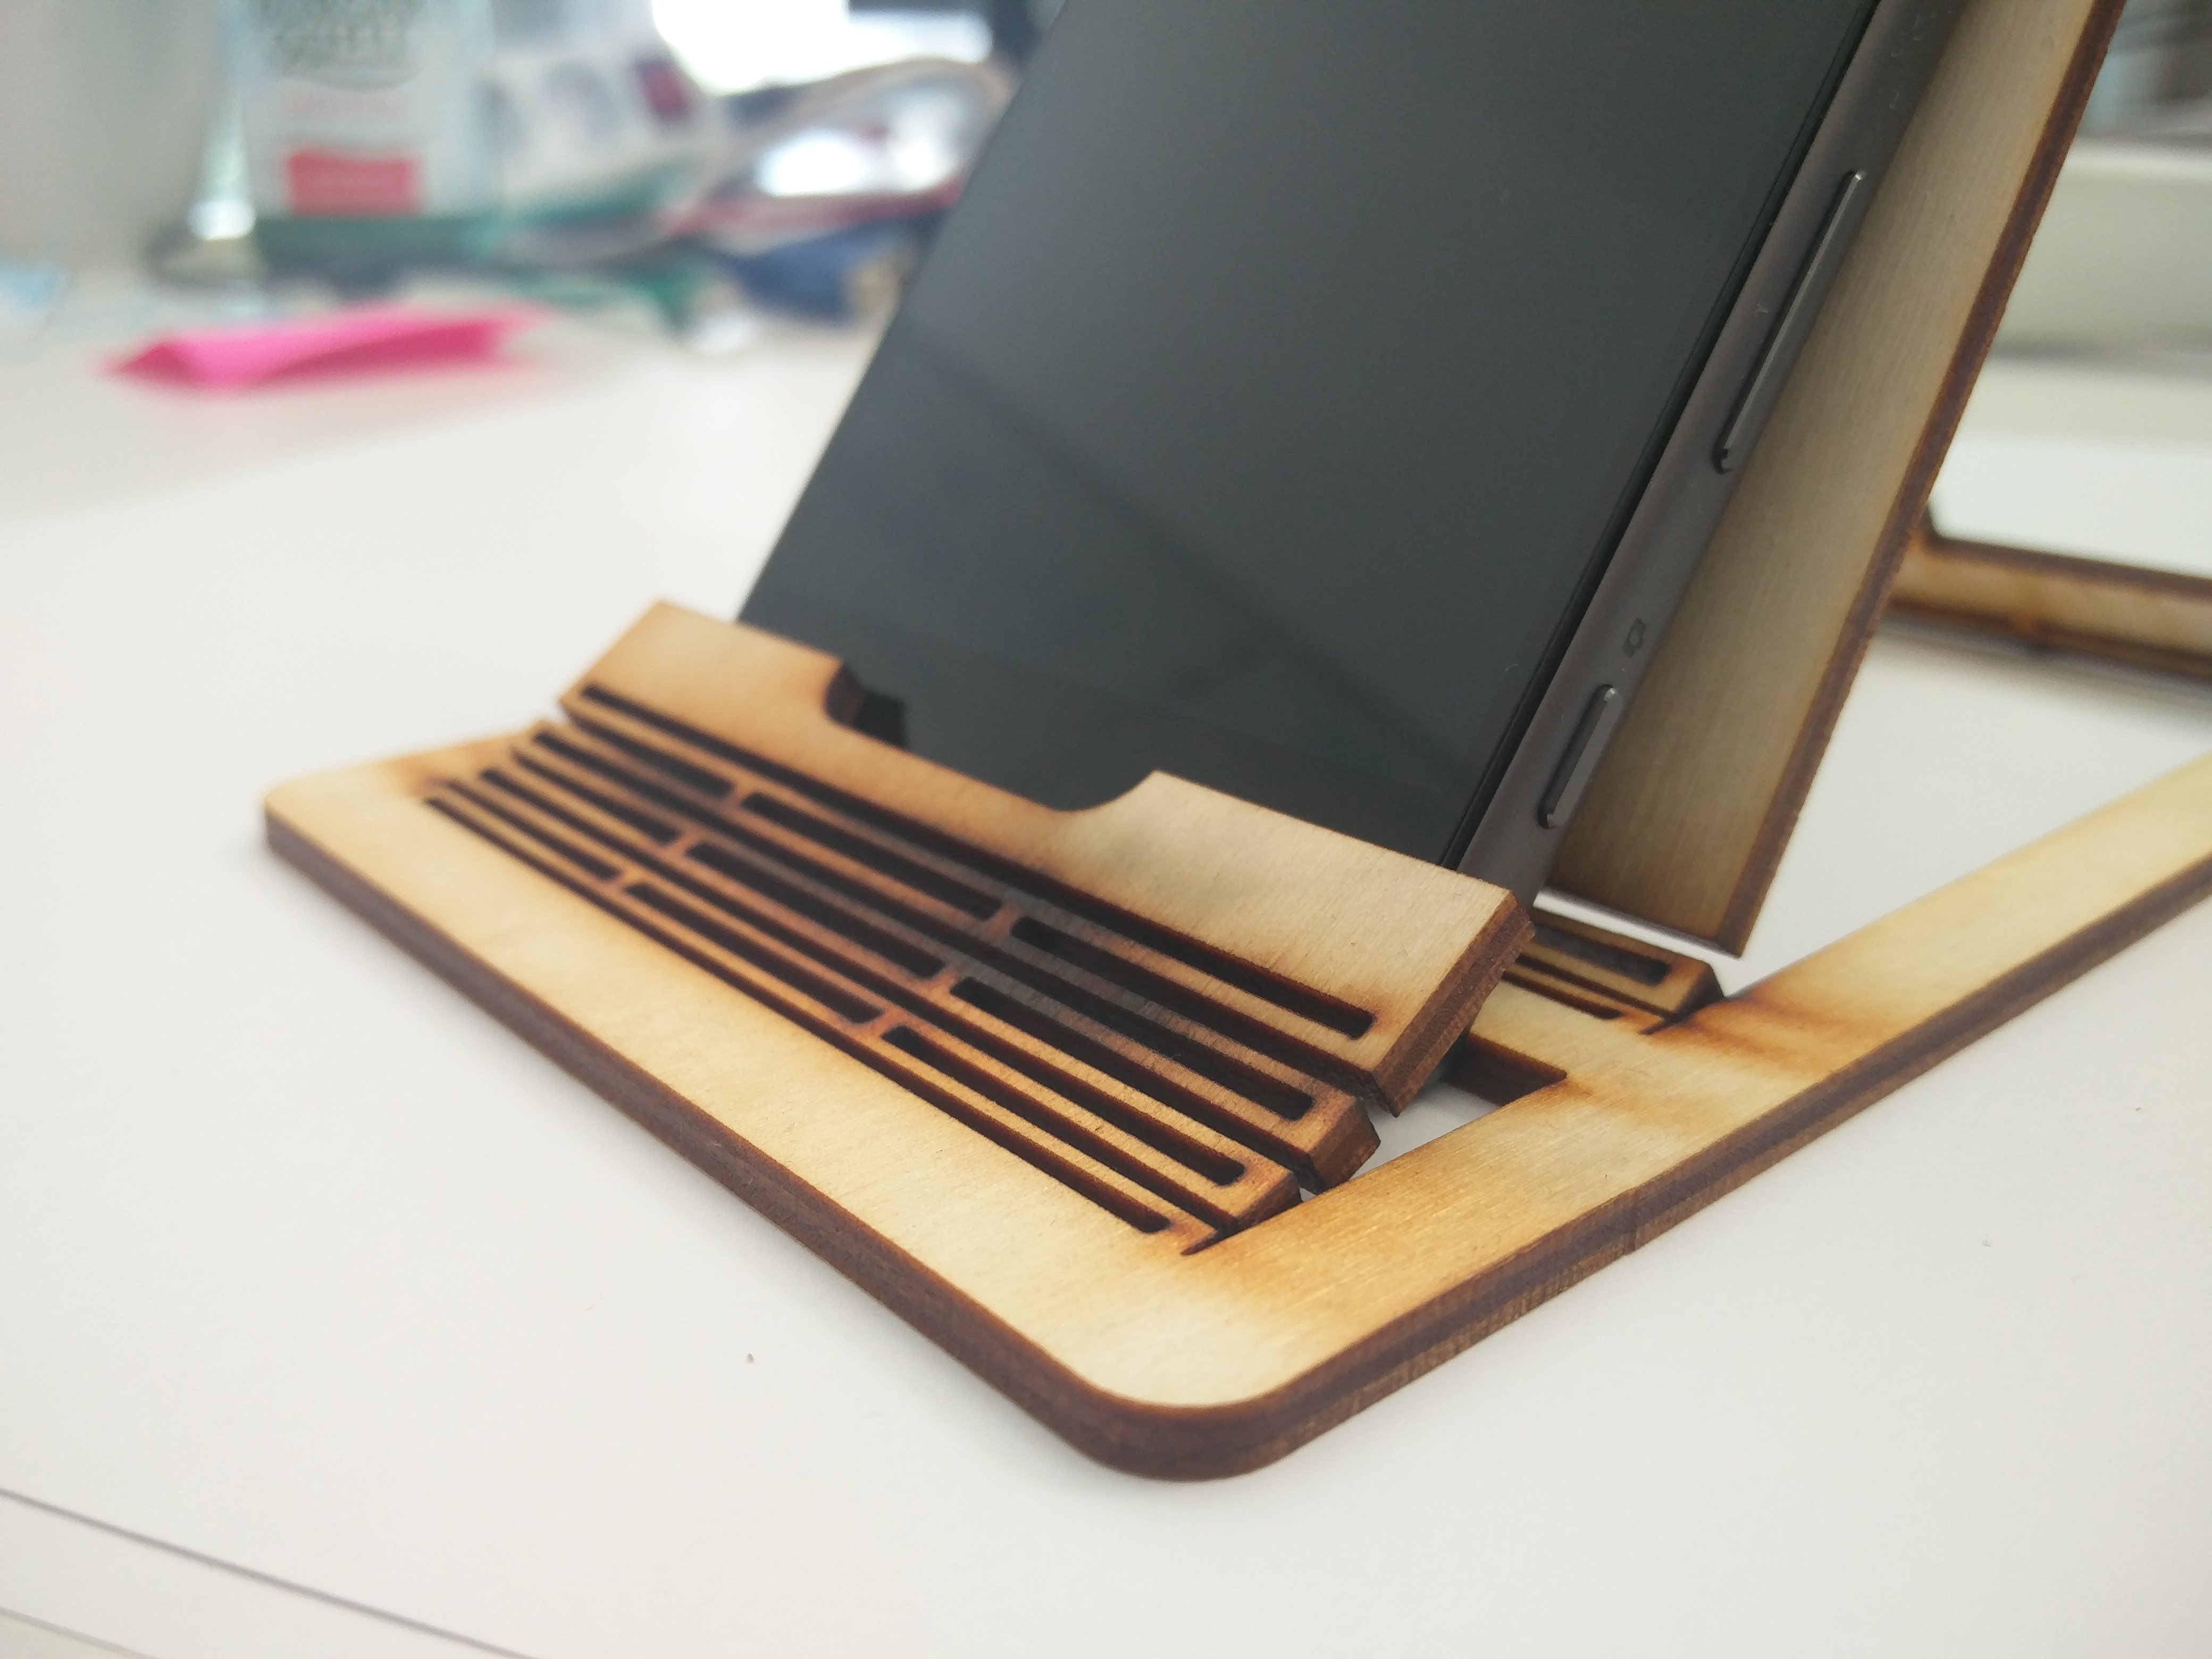
\includegraphics[width=1\textwidth]{07-living_hinge_wood}
    \caption{Laser cut living hinges in a wooden smart phone stand.}
  \end{subfigure}
  \caption{Two typical types of living hinges.}
  \label{fig:living_hinge}
\end{figure}

\section{Developable Surfaces Can be Bend}

Formally developable surfaces are defined as surfaces with zero Gaussian curvature. Practically this means they can be created from a flat surface by cutting, bending and folding and without compressing or stretching. Examples for objects with and without developable surfaces are shown in Figure~\ref{fig:developable_surface_examples}.

\begin{figure}[h]
  \centering
  \begin{subfigure}[b]{0.49\textwidth}
    \centering
    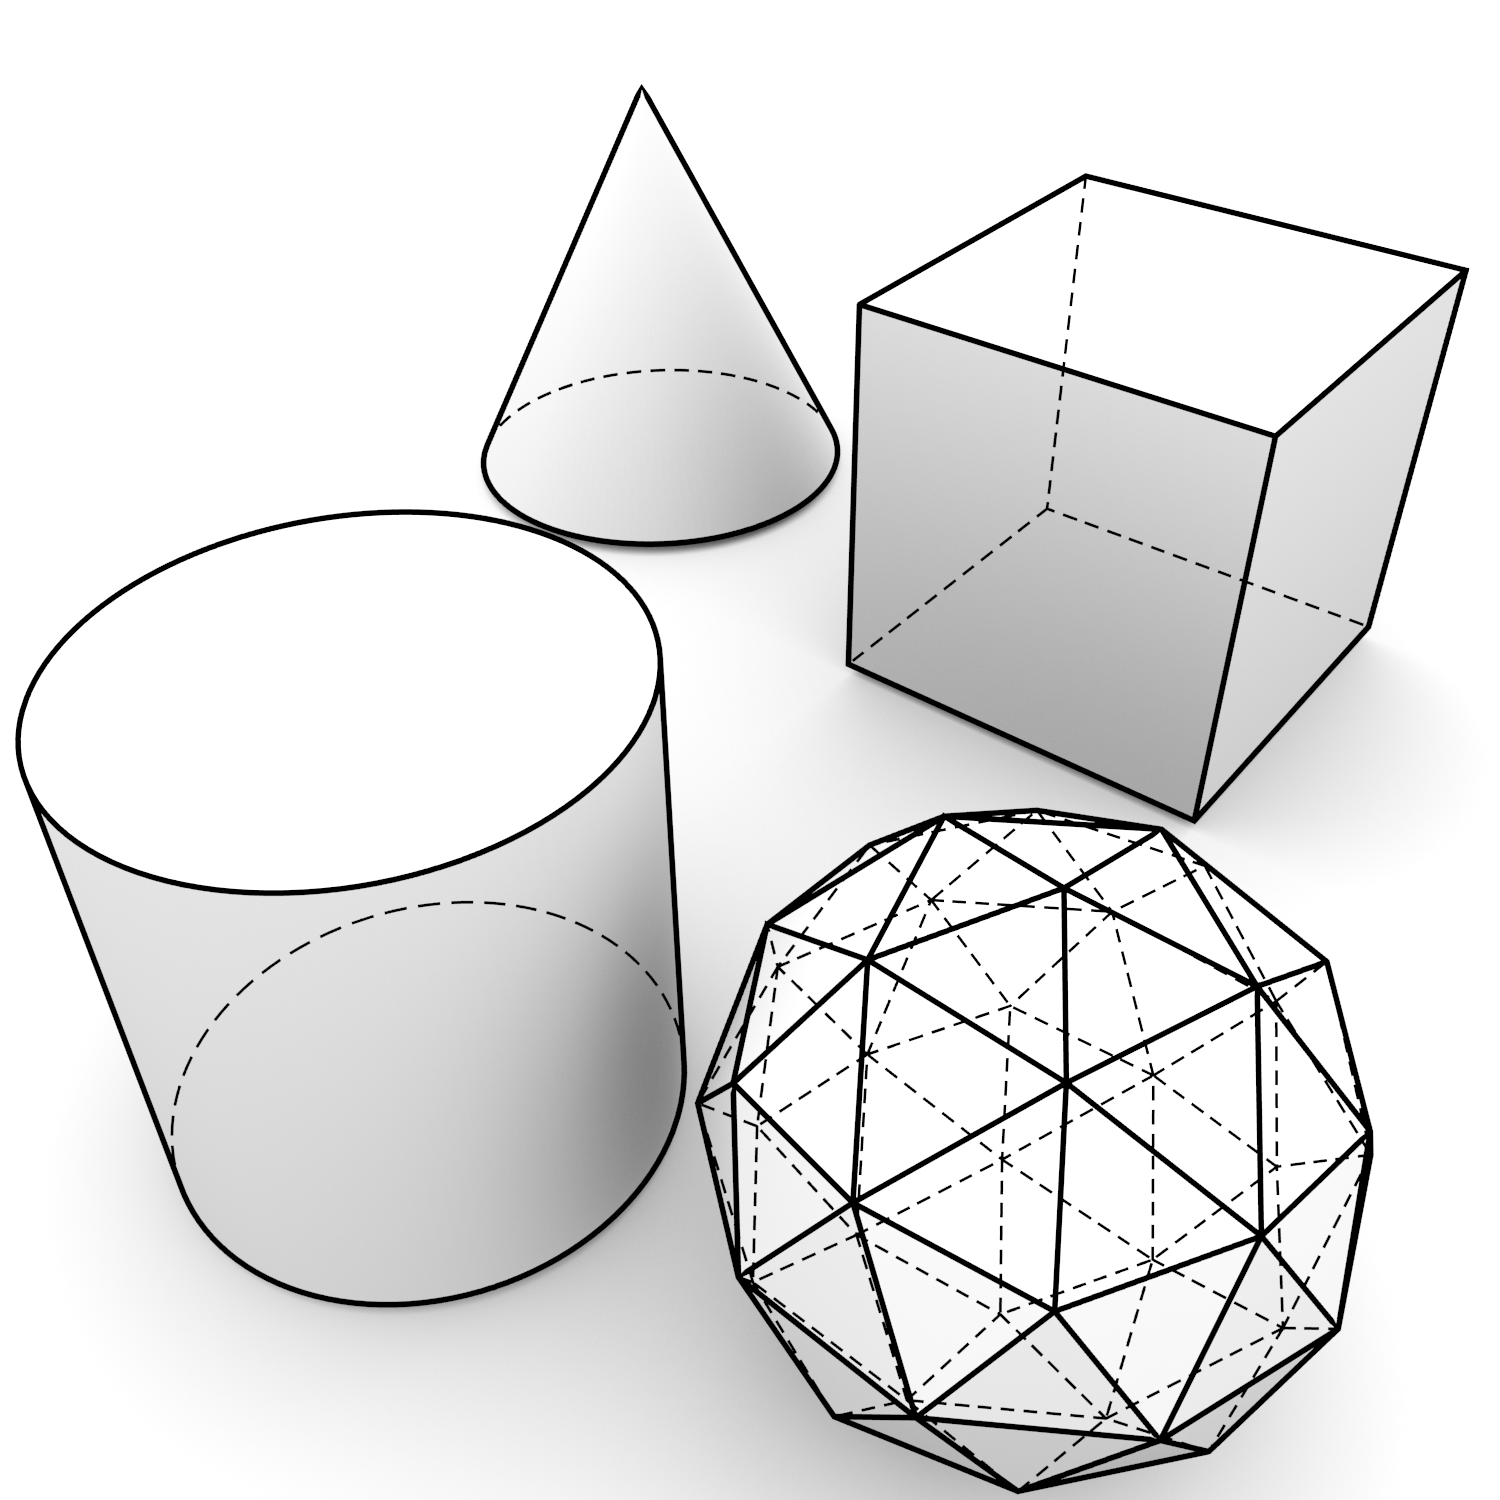
\includegraphics[width=\textwidth]{07-developable_surfaces}
    \caption{Objects like cubes, cylinders, cones and also sphere approximations like an icosphere have developable surfaces.}
  \end{subfigure}
  \begin{subfigure}[b]{0.49\textwidth}
    \centering
    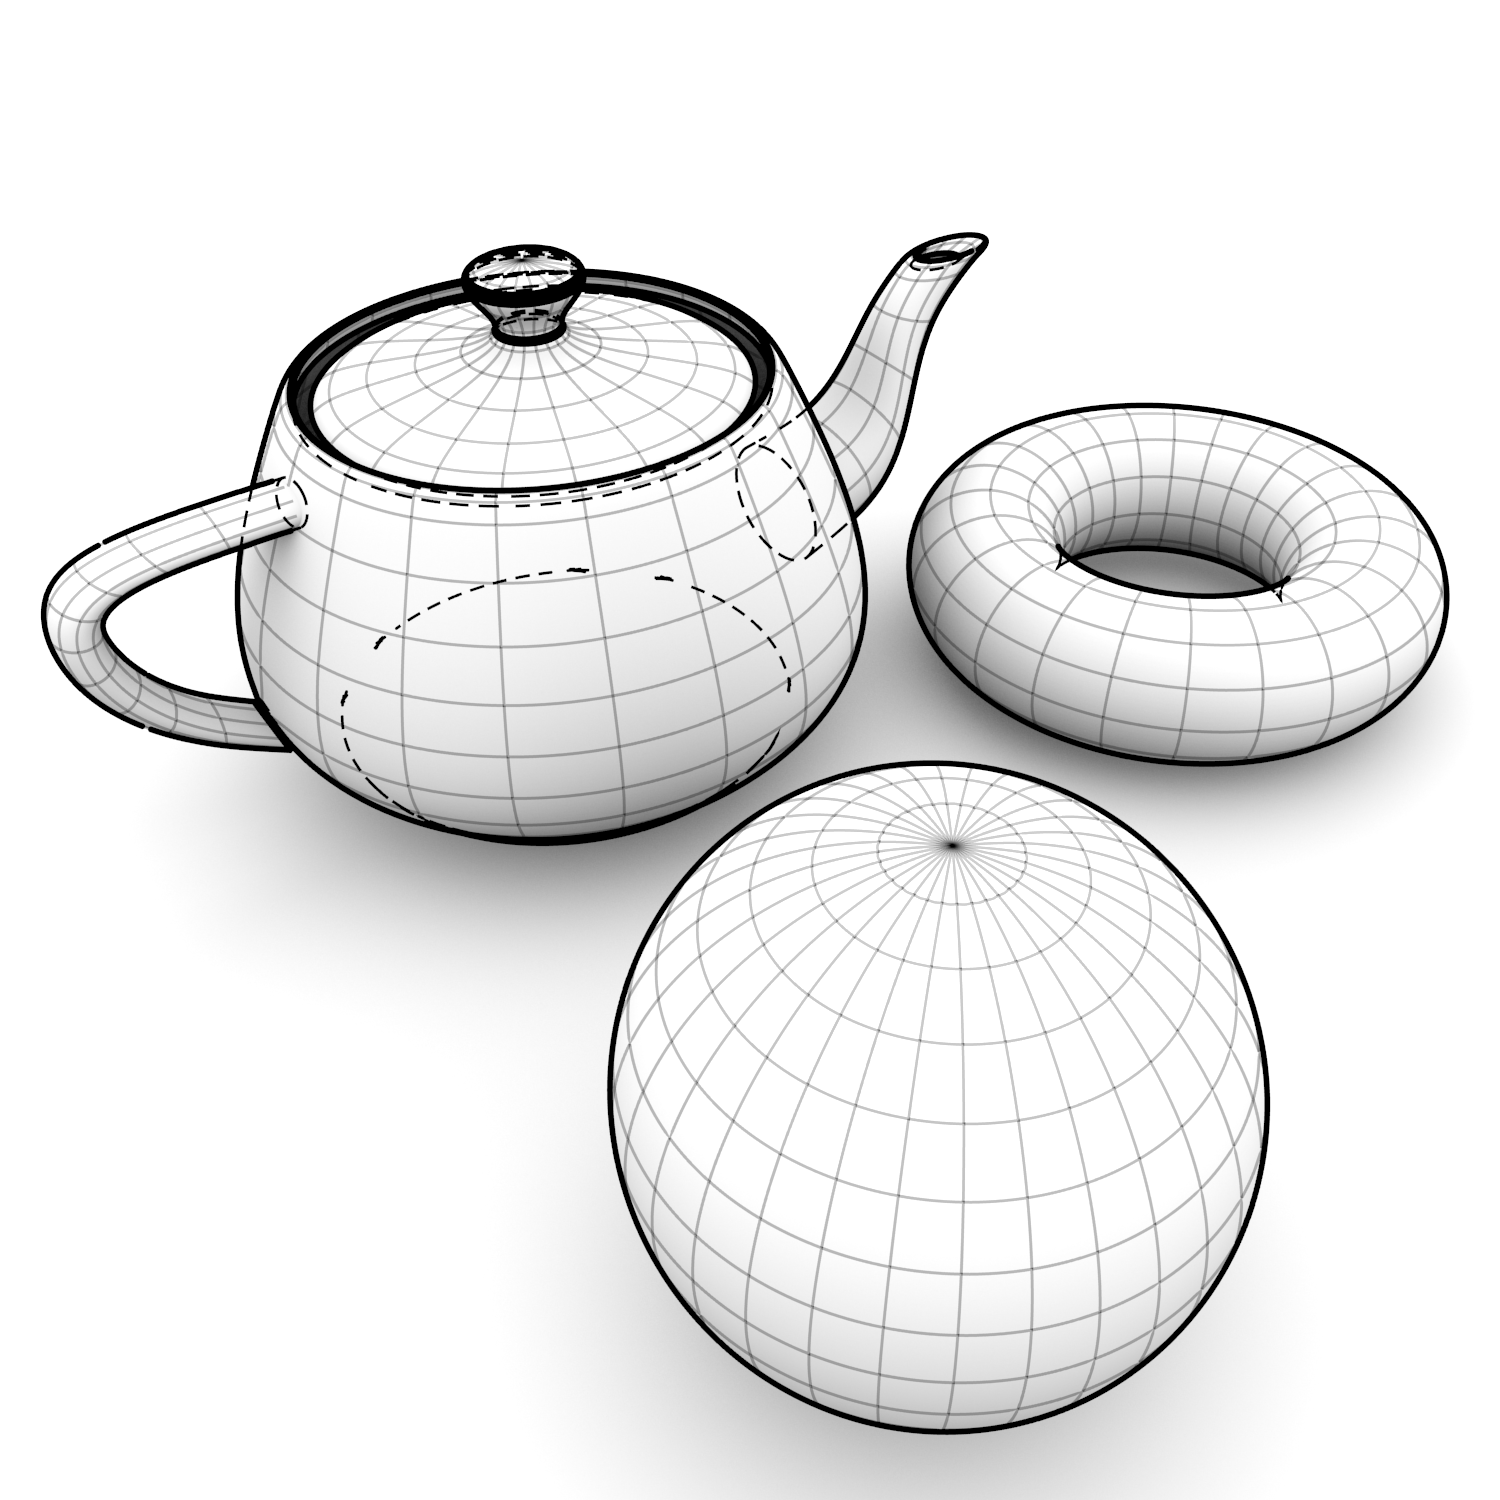
\includegraphics[width=1\textwidth]{07-not_developable_surfaces}
    \caption{So called doubly curved surfaces like from a sphere or torus are not developable.}
  \end{subfigure}
  \caption{Two typical types of living hinges.}
  \label{fig:developable_surface_examples}
\end{figure}

\section{The Bent Plate Object}

\class{Bent plate} is a data structure we use to represent a set of plates which are connected directly or indirectly with bend connections. Thus a bent plate can be cut as one piece. A \class{bent plate} consists of a set of \class{plates}. It provides the method \mintinline{coffeescript}{generateShape} which develops the surface of the connected shapes (see Section~\sectionref{sec:generateShape}). Another method implemented by \class{bent plate} is \mintinline{coffeescript}{generateBendLines} which creates cuttable marks where two plates are merged (see Section~\sectionref{sec:generateBendLines}).

\subsection{The GenerateShape Function Creates a Shape of the Developed Surface}
\label{sec:generateShape}

To generate the \class{shape} of the \class{bent plate} we first check how many \class{plates} this \class{bent plate} contains. If none are contained, the generated \class{shape} is \emph{null}. If there is just one \class{plate} then its \class{shape} is used.

If there are multiple plates in the bent plate the generation is done the following way: For each of the plates in the bent plate, the corresponding shape is transformed using the bend matrix (see Section~\sectionref{sec:traverse-along-bend-connection}). Afterwards, they are converted into polygons suitable for using with the \jsclipper{} and merged using the \emph{union} function.

To avoid unconnected polygons after merging caused by floating point inaccuracy we use vertex welding before merging (see Section~\sectionref{sec:vertex_welding}). The resulting polygon is converted back to a shape (see Listing~\ref{lst:generateShape}).

\begin{listing}[ht]
\begin{minted}[
linenos,breaklines
]{coffeescript}
generateShape: ->
  if @plates.length < 1
    @shape = null
    return
  if @plates.length is 1
    @shape = @plates[0].shape
    return
  # lay shapes into xy-plane
  polygons = @plates.map (plate) =>
    bentMatrix = plate.bentMatrix
    shape = plate.shape
    contour = @applyMatrices(
      shape.getContour(), bentMatrix)
    holes = shape.getHoles().map (hole) =>
      @applyMatrices hole, bentMatrix
    return {contour, holes }
  # remove-doubles-fix
  weldingDistance = 0.02
  welder = new VertexWelding(weldingDistance)
  polygons.forEach (polygon) ->
    polygon.contour.forEach (vertex) ->
    correspondingVertex = welder.getCorrespondingVertex(
      {x: vertex[0], y: vertex[1], z: 0})
    vertex[0] = correspondingVertex.x
    vertex[1] = correspondingVertex.y
  # create clipping polygons
  polygons = polygons.map (polygon) ->
    return new Clipper.Polygon(
      polygon.contour, polygon.holes)
  # merge polygons
  mergedPolygon = polygons[0]
  polygons.shift()
  mergedPolygon = mergedPolygon.unionMultiple polygons
  # create shape from clipping polygon
  contour = mergedPolygon[0].getShape().map (vertex) ->
    return new THREE.Vector3 vertex[0], vertex[1], 0
  contour = new EdgeLoop contour
  holes = mergedPolygon[0].getHoles().map (hole) ->
    hole = hole.map (vertex) ->
    return new THREE.Vector3 vertex[0], vertex[1], 0
    hole = new EdgeLoop hole
    hole.hole = true
    return hole
  shape = holes
  shape.push contour
  shape = new Shape shape, new THREE.Vector3 0, 0, 1
  # set shape as shape of the bent plate
  @shape = shape
\end{minted}
\caption{Generating the shape for a bent plate.}
\label{lst:generateShape}
\end{listing}

\subsection{Bend Lines Help to Bend the Plate}
\label{sec:generateBendLines}

This method generates a dashed line located at the connection line between two plates of the bent plate. This marks where the user must bend the material. Additionally, it weakens the material and allows for easier bending.

To locate the general placement of the bend line all intersection lines of the bent plate are processed. They are checked whether they belong to a bend connection and are not used for creating a bend line yet. To place them into the shape they are transformed by the corresponding bend matrix (see Listing~\ref{lst:generateBentLines}).

\begin{listing}[ht]
\begin{minted}[
linenos,breaklines
]{coffeescript}
generateBendLines: ->
  seenConnections = []
  @bendLines = []
  polygons = @plates.forEach (plate) =>
    bentMatrix = plate.bentMatrix
    plate.connectionList.forEach (connection) =>
      parameters = connection.parameters
      if parameters.joint is 'bend' and not (parameters in seenConnections)
        seenConnections.push parameters

        intersectionLine = parameters.intersectionLine.clone()
        intersectionLine.applyMatrix4 bentMatrix
        intersectionLine.start.z = 0
        intersectionLine.end.z = 0
        @generateDashedLines intersectionLine

        @bendLines.push intersectionLine
\end{minted}
\caption{Generate the bend lines for a bent plate.}
\label{lst:bend-matrix}
\end{listing}

At this position we create a dashed cutting line.

\section{Setting the Joint Type}

In this step, we try to find out which connections can be implemented as a bending joint. The resulting shape of the connected plates is developable without overlaps. The difference between a model which surface is developable without overlaps and one which in not is shown in Figure~\ref{fig:overlaps}.

\begin{figure}[h]
  \centering
  \begin{subfigure}[b]{0.49\textwidth}
    \centering
    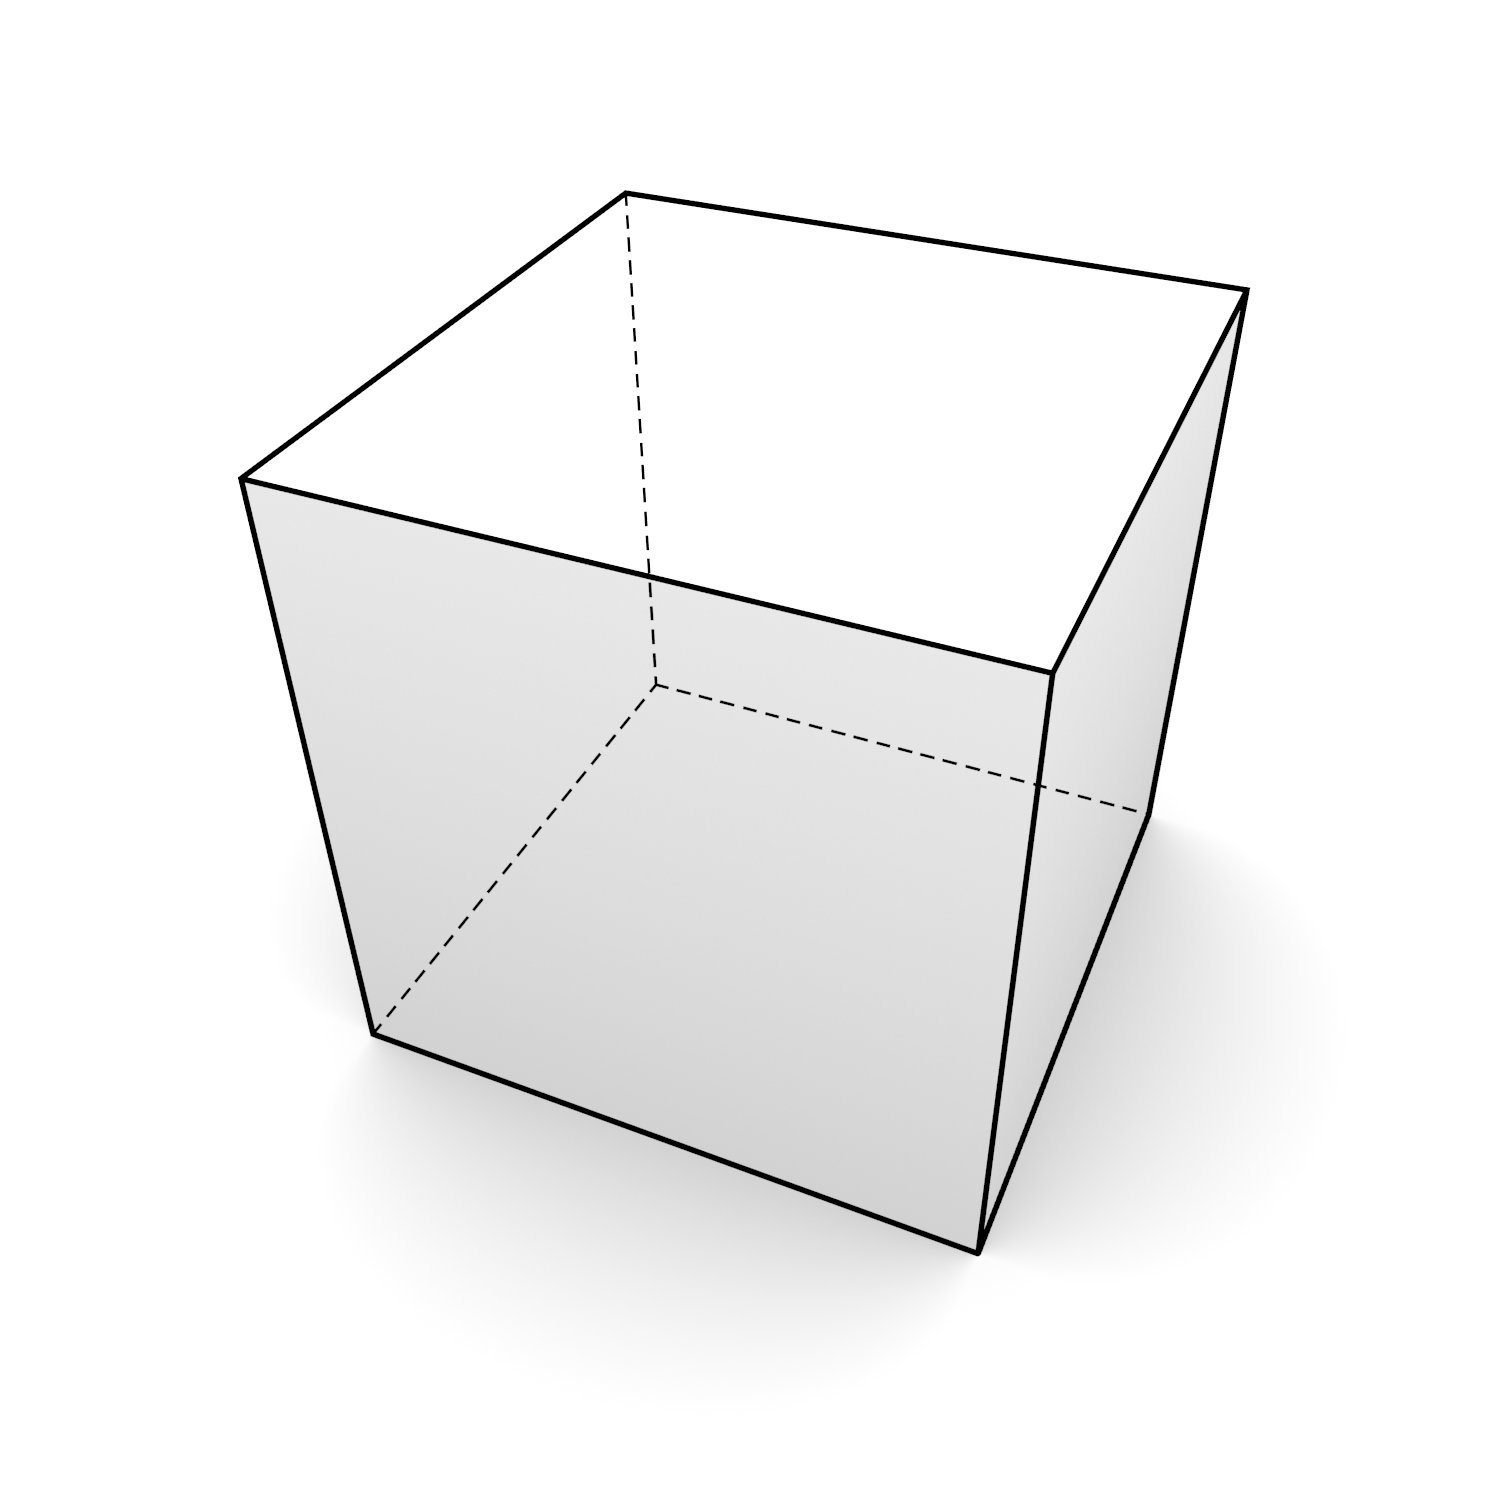
\includegraphics[width=\textwidth]{07-no_overlaps}
    \caption{A cubes' surface can be developed without overlaps.}
    \label{fig:overlaps:no-3d}
  \end{subfigure}
  \begin{subfigure}[b]{0.49\textwidth}
    \centering
    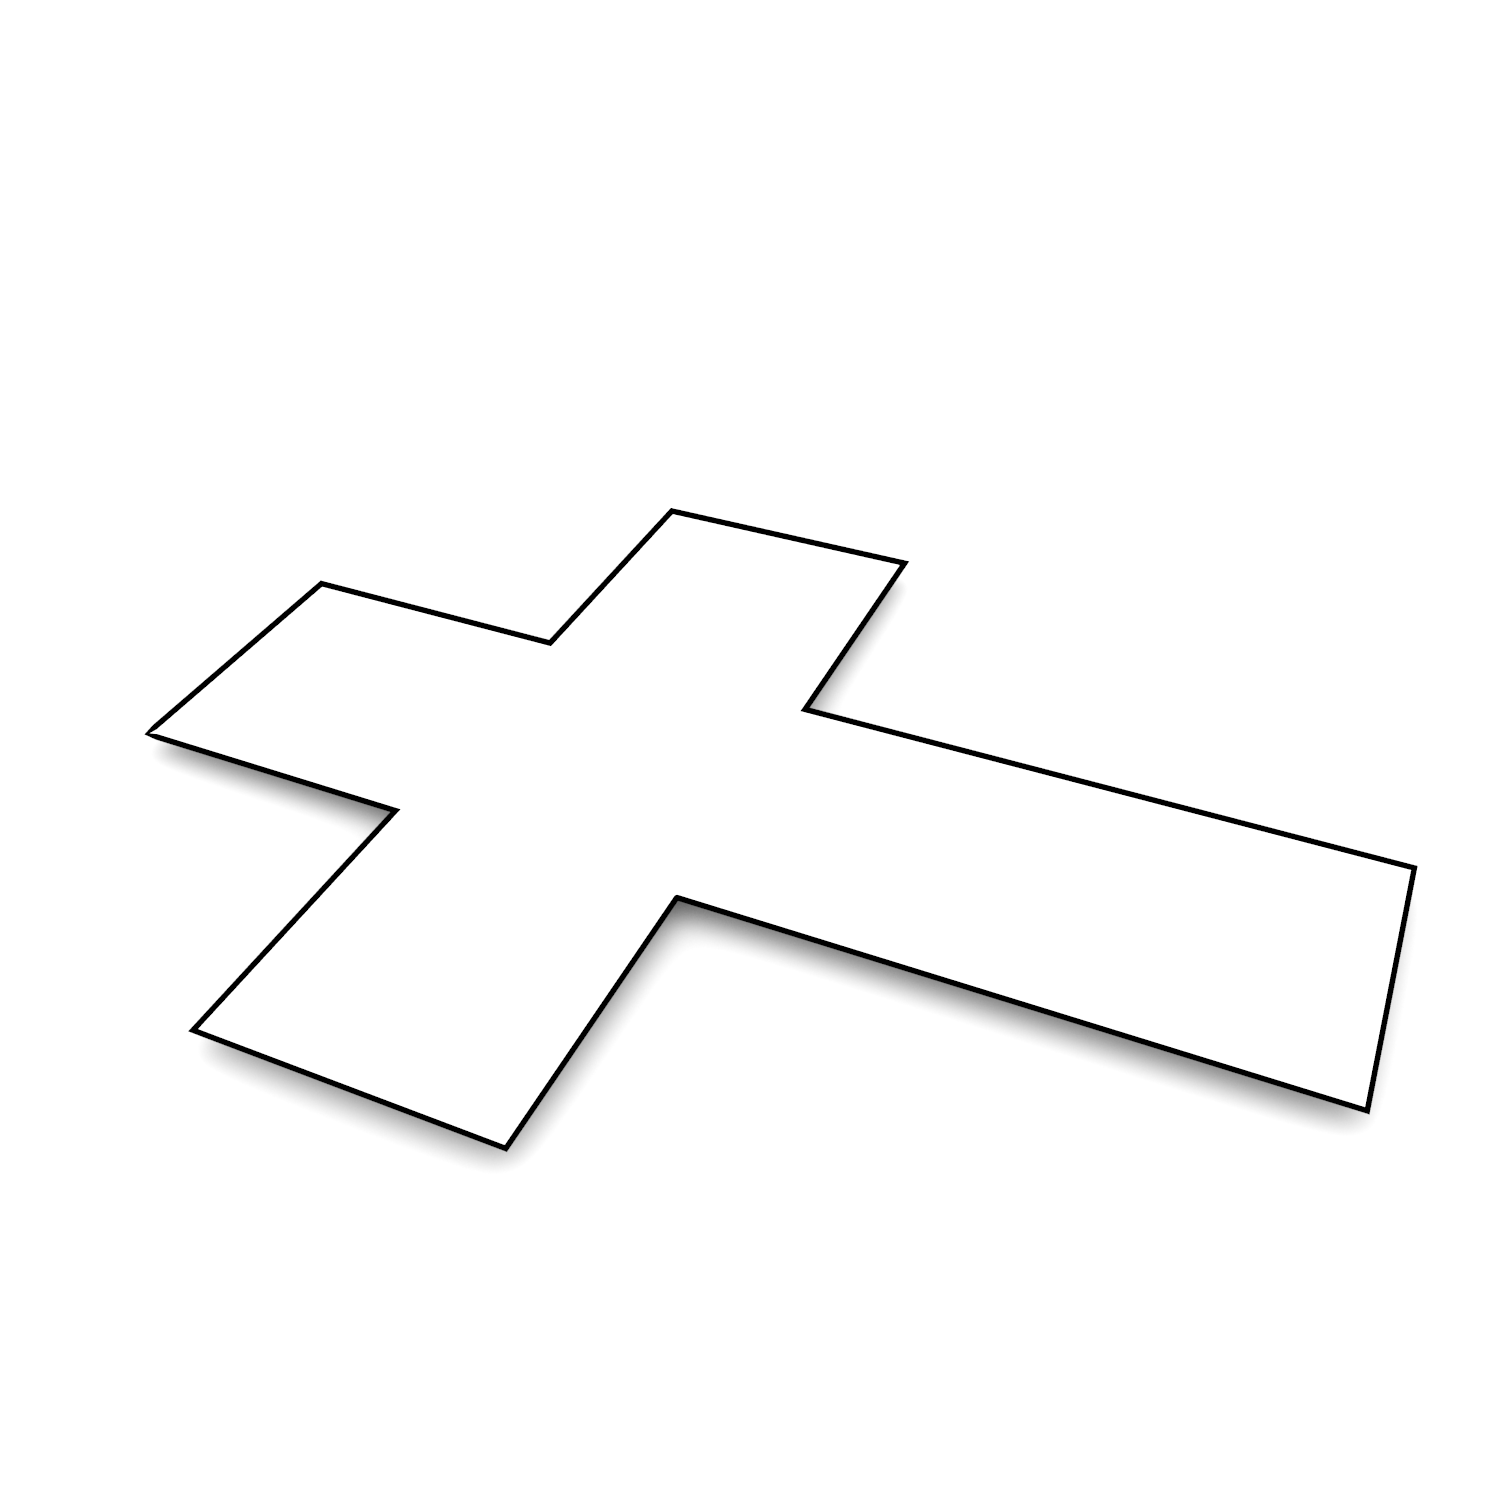
\includegraphics[width=1\textwidth]{07-no_overlaps_2d}
    \caption{One possible developed surface of a cube.}
    \label{fig:overlapsh:no-2d}
  \end{subfigure}
  \begin{subfigure}[b]{0.49\textwidth}
    \centering
    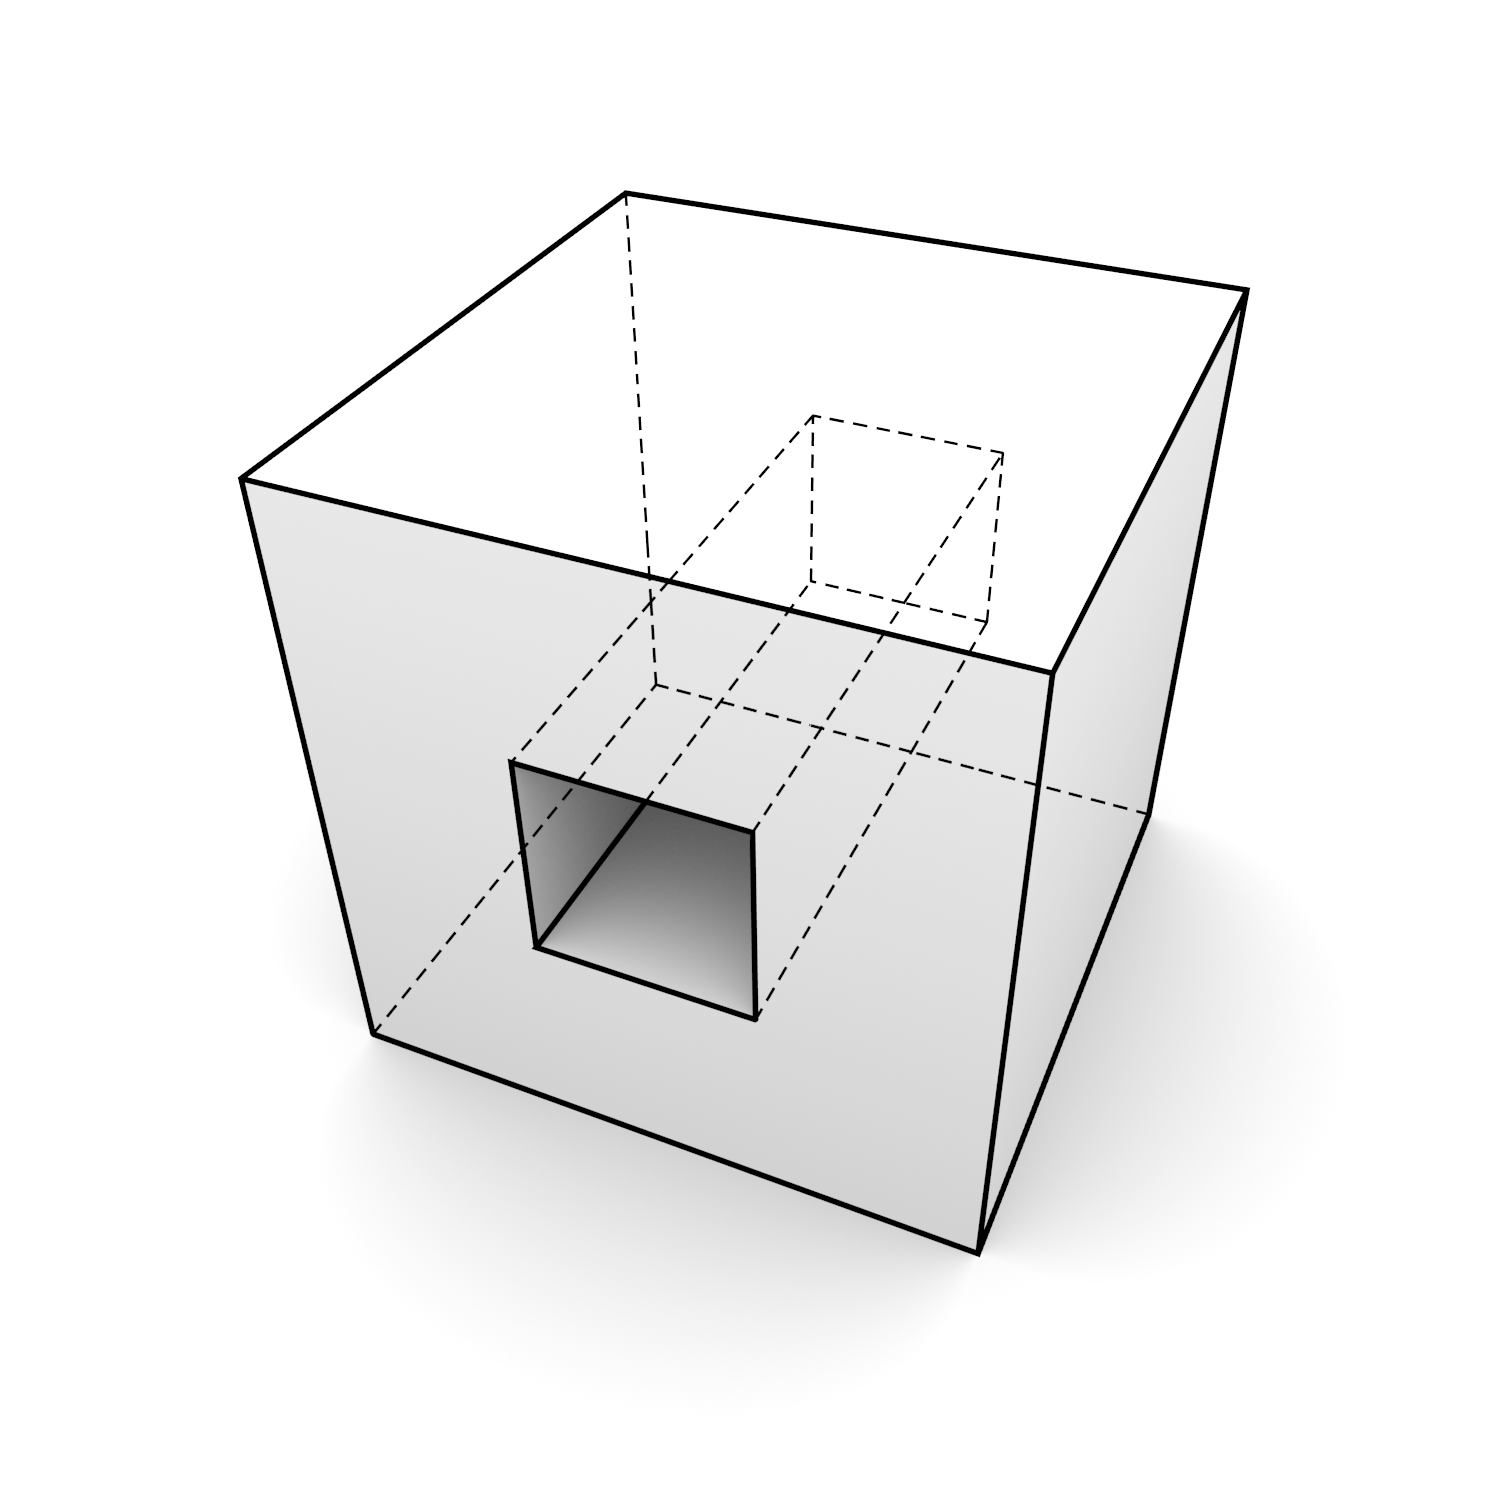
\includegraphics[width=\textwidth]{07-overlaps}
    \caption{The surface of a cube with a hole can not be developed without overlaps.}
    \label{fig:overlaps:some-3d}
  \end{subfigure}
  \begin{subfigure}[b]{0.49\textwidth}
    \centering
    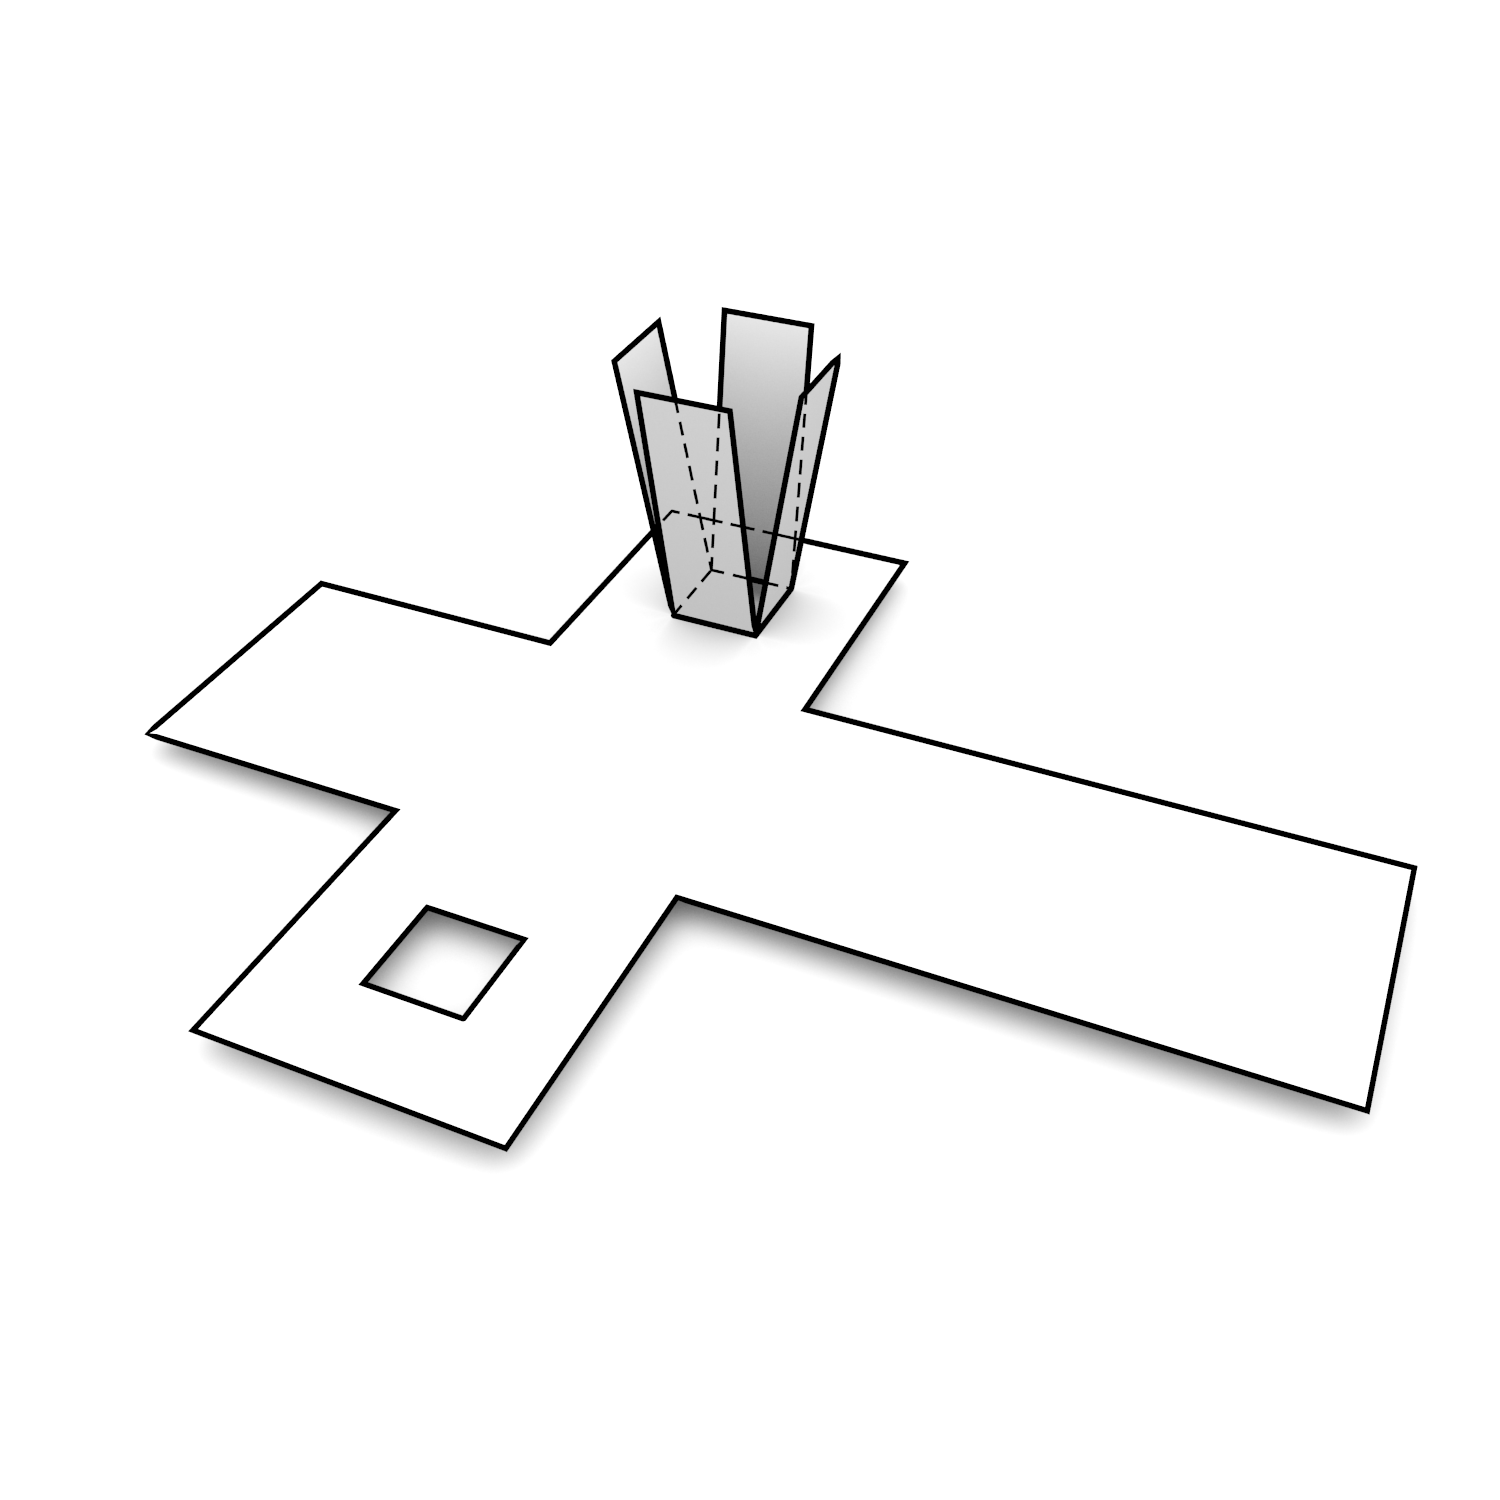
\includegraphics[width=1\textwidth]{07-overlaps_2d}
    \caption{The shapes inside the hole will always overlap some part of the developed surface.}
    \label{fig:overlaps:some-2d}
  \end{subfigure}
  \caption{Two objects with a developable surface, but one without and one with overlaps.}
  \label{fig:overlaps}
\end{figure}

To do so, we start with one plate and run a series of tests for all of its connections:
\begin{itemize}
\item Is the type of this connection not yet set (it is set to \emph{unset} instead of e.g. \emph{bend joint})?
\item Is the connection angle close enough to 180\textdegree{}, allowing the material to be bent this far? (What near enough means depends on the used material see Section~\sectionref{sec:material_dependant_bend_angle})
\item Is it possible to add the to-be-connected plate's shape to the currently processed plate's shape without overlapping?
\end{itemize}
If all checks succeed, the connected plate is added to this plate and they form a bent plate. If the connection type is not yet set but one of the other tests fails a finger joint is used.

This is repeated for all the connections of the bent plate until we assigned a joint type to each of them. This process is repeated until all plates are assigned to a bent plate.

%shorten this sentence:
When checking if a plate could be added to an existing bent plate, two shapes are created. The first one is the union of the bent plate's shape and all of its finger joint shapes, excluding the connection with the new plate. The second is the union of the shape of the new plate and its finger joint shapes, excluding the connection with the bent plate.

Afterwards, we calculate the intersection of this two. If the result is empty, there are no overlaps, the plate can be safely added to the bent plate. The connection is annotated as a bending joint.

%If one of the conditions is not fulfilled the connection can not be a bend and is annotated as finger joint.

\section{Building the Bent Plates}
%TODO find subsection title
For building the bent plates our implementation starts with one plate of the plate graph and traverses the graph along the marked bend connections. This way all directly or indirectly connected plates (via bend connections) are collected into a array. From these plates one bent plate is created. If there are plates in the plate graph which are not added to a bent plate, the process is repeated until no plate is left.

\subsection{Traversing Along Bend Connections}
\label{sec:traverse-along-bend-connection}

While traversing along the bend connections, the transformation matrices for the plates are calculated.

The first plate's matrix is already known. It is the rotation matrix of its shape to rotate it into the xy-plane.

When laying the other plates into the xy-plane, it is important to make sure that they keep touching with the connected plate while laying them into this plane. Therefore the bend angle must be calculated. It is 180\textdegree{} minus the angle between the connected plates, which is already known from the plate graph creation.

The bend axis is the axis  to rotate around to develop the surface. It is determined by calculating the cross product of the two normals of the connected plates. This way the axis does not only lie at the right place but also points in the right direction (This would not be the case if only the connection line between the two plates is used).

The axis has to be transformed into the xy-plane, onto the edge of the previous plate. To do so, our implementation uses the starting point of the intersection line and ending point, which is created by adding the axis vector to the starting point. These two points are transformed using the transformation matrix of the previous plate. The final axis is determined from the transformed points by subtracting the ending point form the staring point.

The angle and the axis are used to create the rotation matrix used to lay the plate in the same plane like the previous one.

Because the rotation matrix only rotates around the point of origin, two translation matrices are created. The first one translates the plate to the origin after which the rotation is performed to lay the plate into the xy-plane. The second one translates the plate back to the connection edge.

For calculating the final transformation matrix for this plate, the transformation matrix of the previous plate is multiplied by the first translation matrix, the rotation matrix and finally the second translation matrix. This will also be used for creating the transformation matrices of the following plates.

\begin{figure}[h]
  \centering
  \begin{subfigure}[b]{0.49\textwidth}
    \centering
    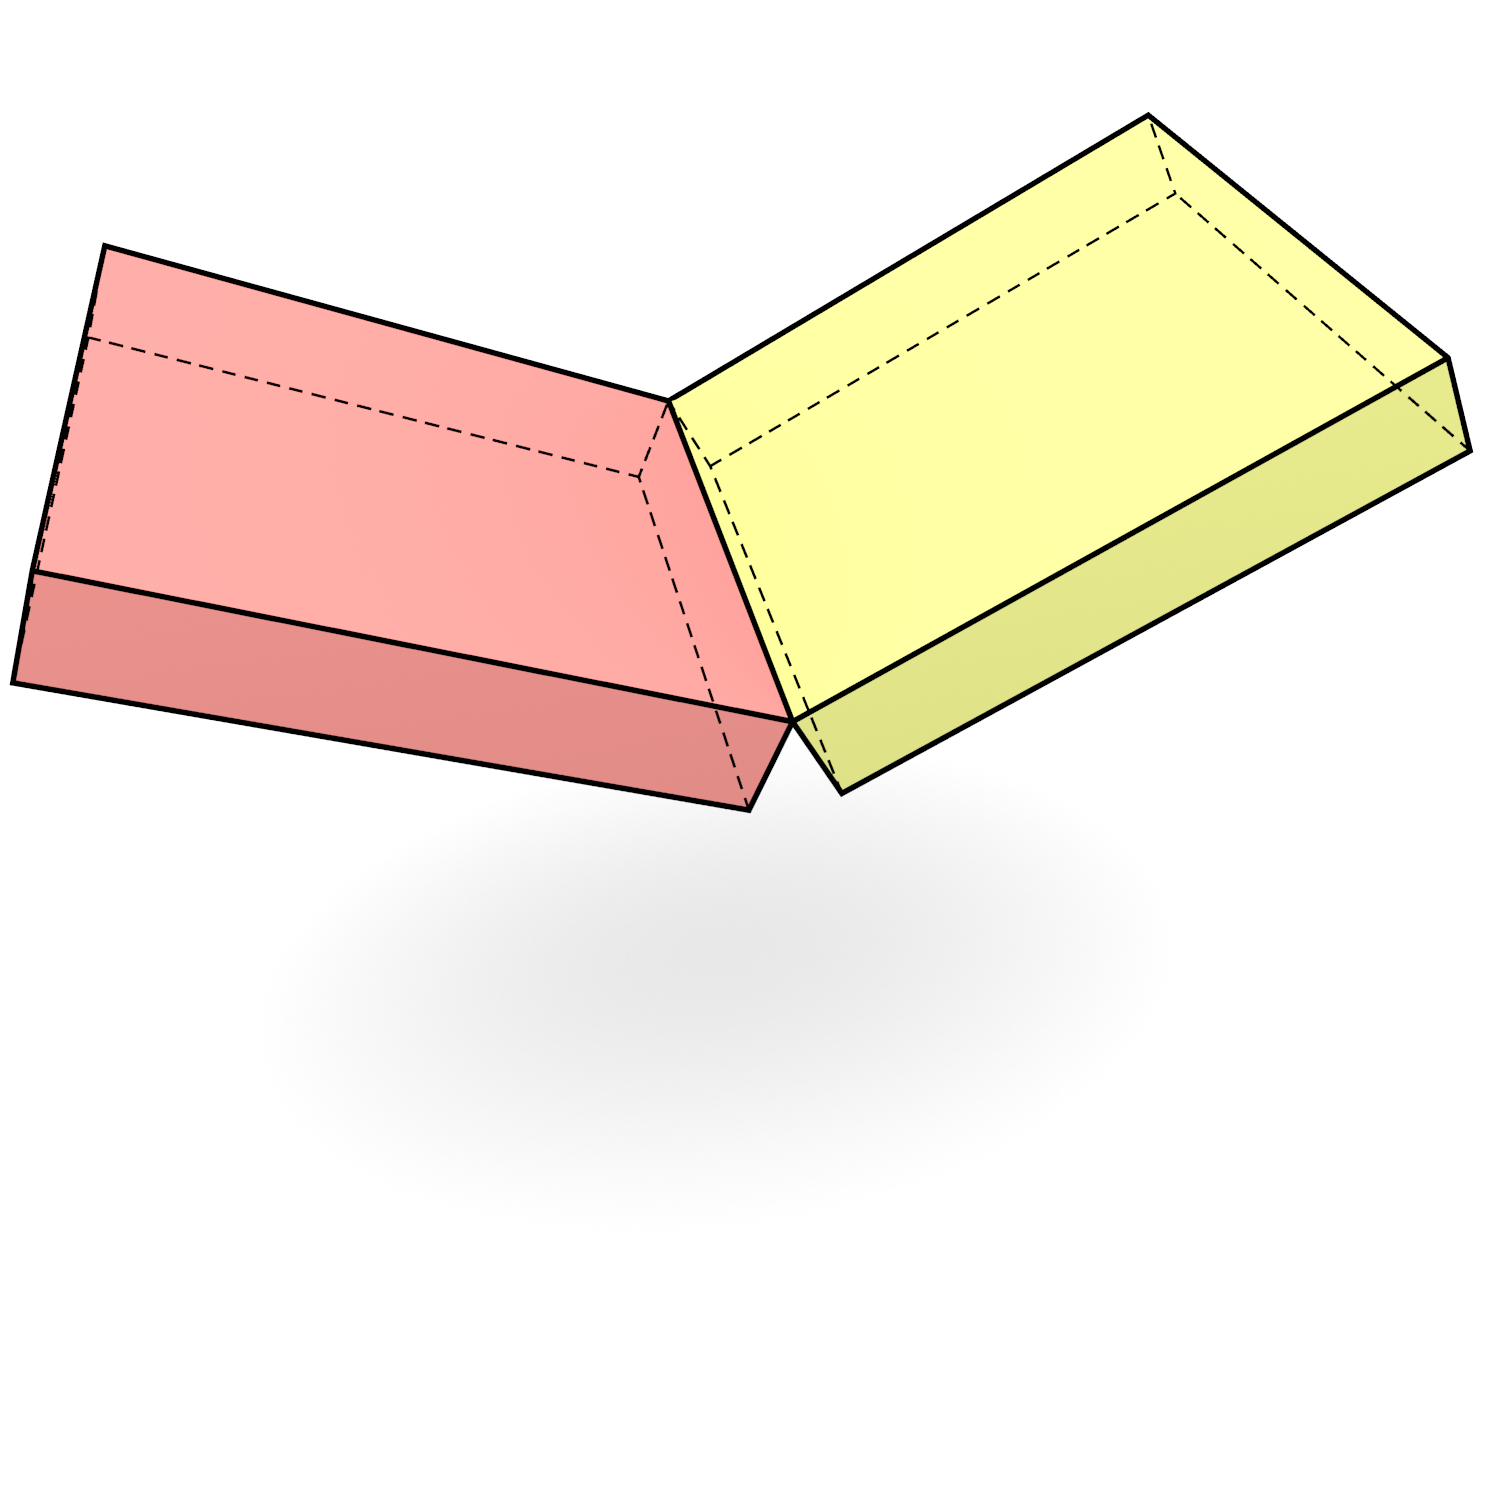
\includegraphics[width=\textwidth]{07-traversing_along_bend_connections_01}
    \caption{Two plates which should be connected with a bend.}
    \label{fig:bend-matrix:1}
  \end{subfigure}
  \begin{subfigure}[b]{0.49\textwidth}
    \centering
    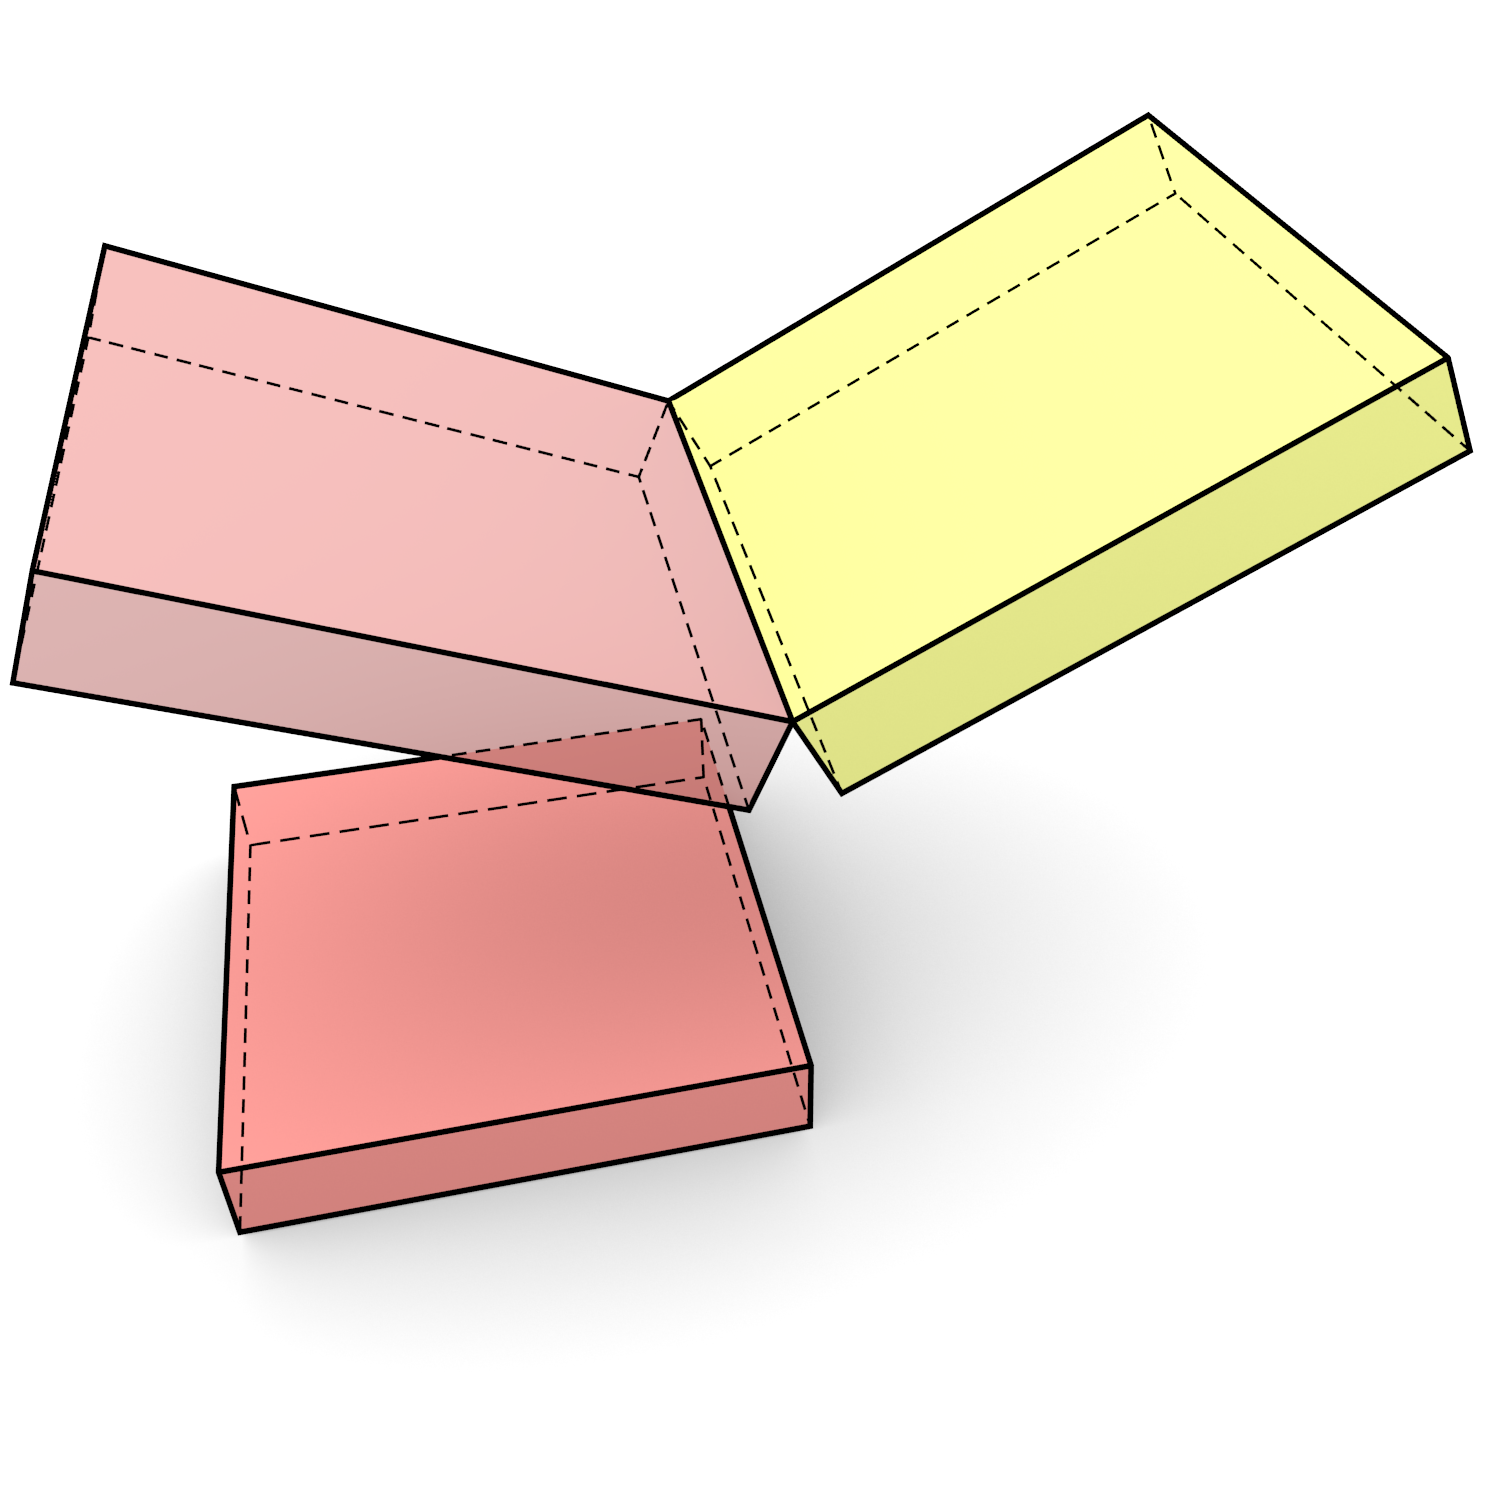
\includegraphics[width=1\textwidth]{07-traversing_along_bend_connections_02}
    \caption{For the first one the transformations matrix is known already.}
    \label{fig:bend-matrix:2}
  \end{subfigure}
  \begin{subfigure}[b]{0.49\textwidth}
    \centering
    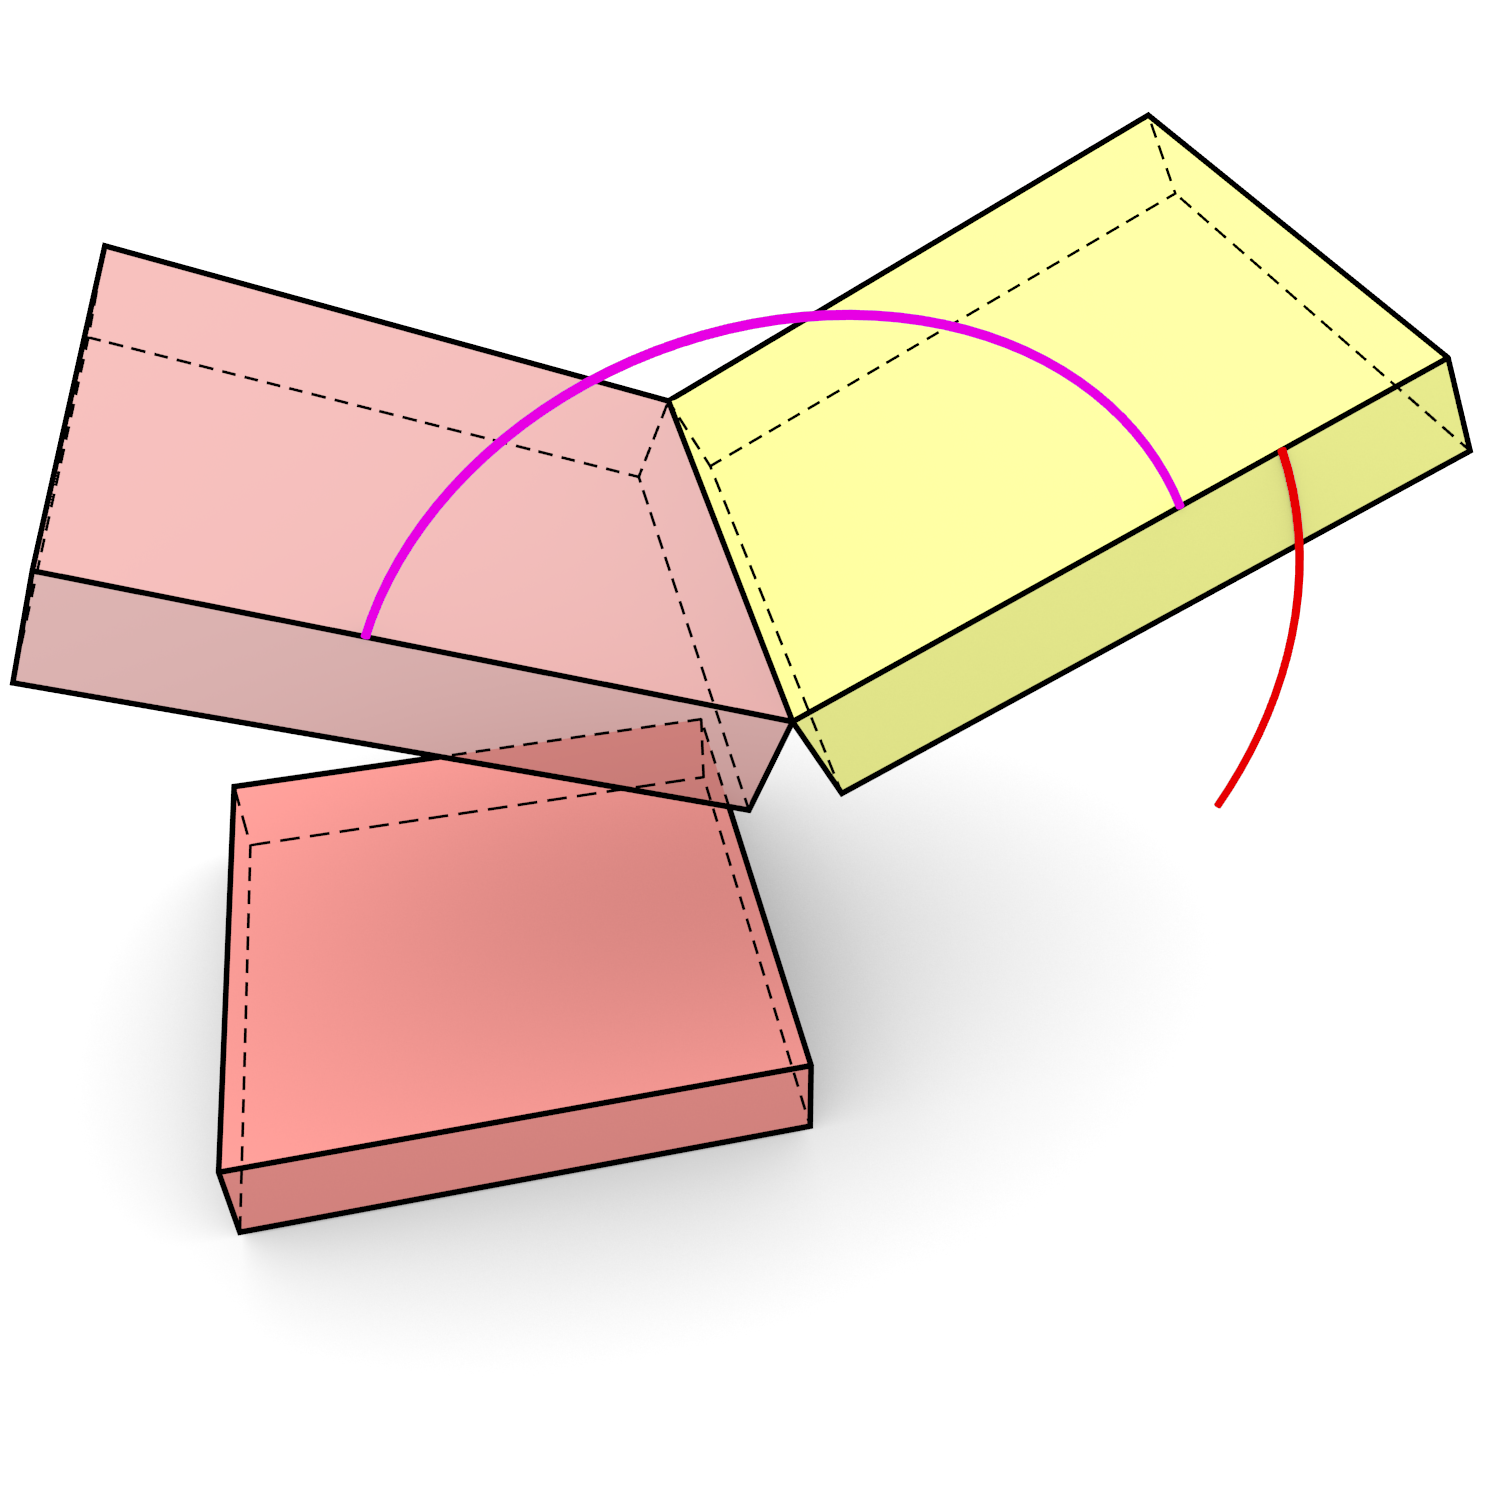
\includegraphics[width=\textwidth]{07-traversing_along_bend_connections_03}
    \caption{The bend angle (red) is 180\textdegree{} minus the angle between the plates (magenta).}
    \label{fig:bend-matrix:3}
  \end{subfigure}
  \begin{subfigure}[b]{0.49\textwidth}
    \centering
    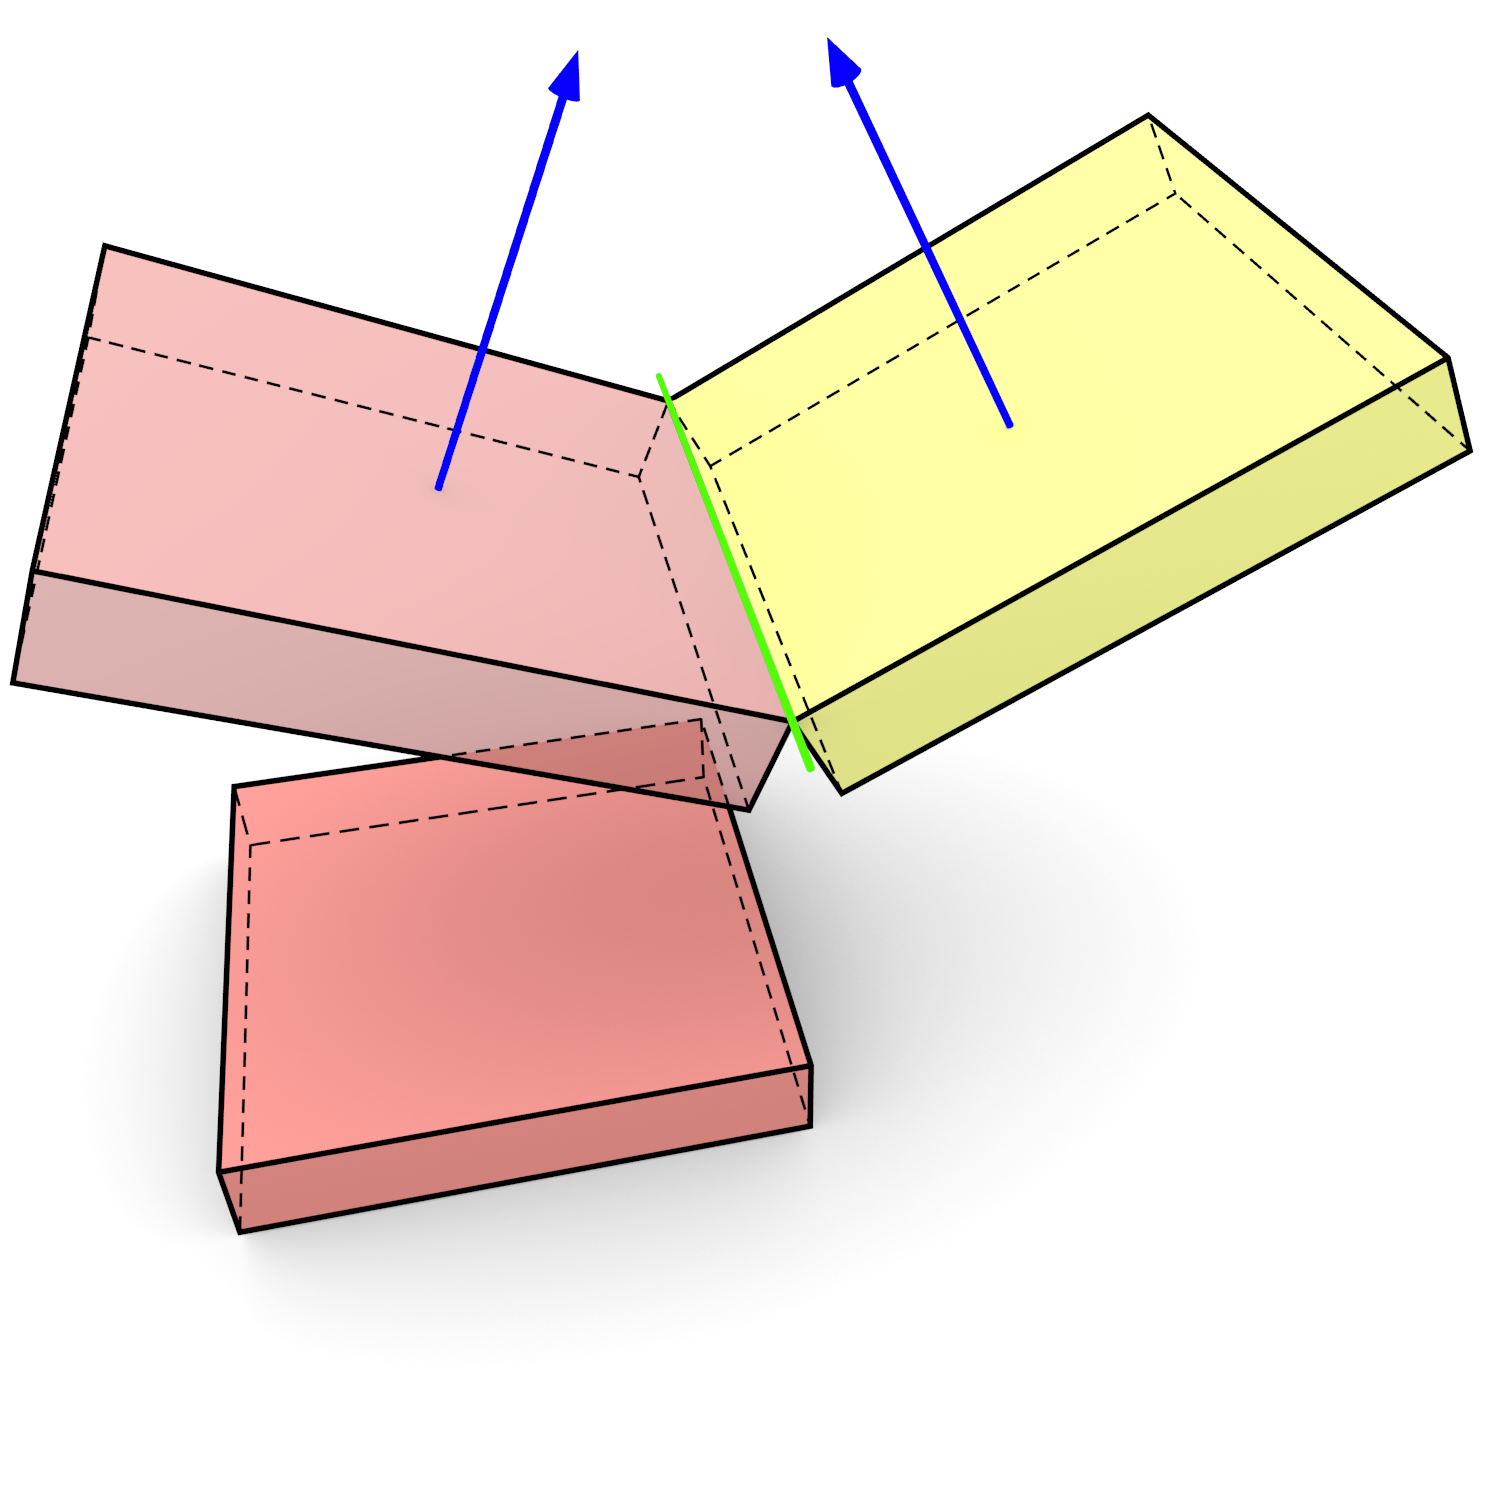
\includegraphics[width=1\textwidth]{07-traversing_along_bend_connections_05}
    \caption{The bend axis is the cross product of the bent plate's normals.}
    \label{fig:bend-matrix:4}
  \end{subfigure}
  \begin{subfigure}[b]{0.49\textwidth}
    \centering
    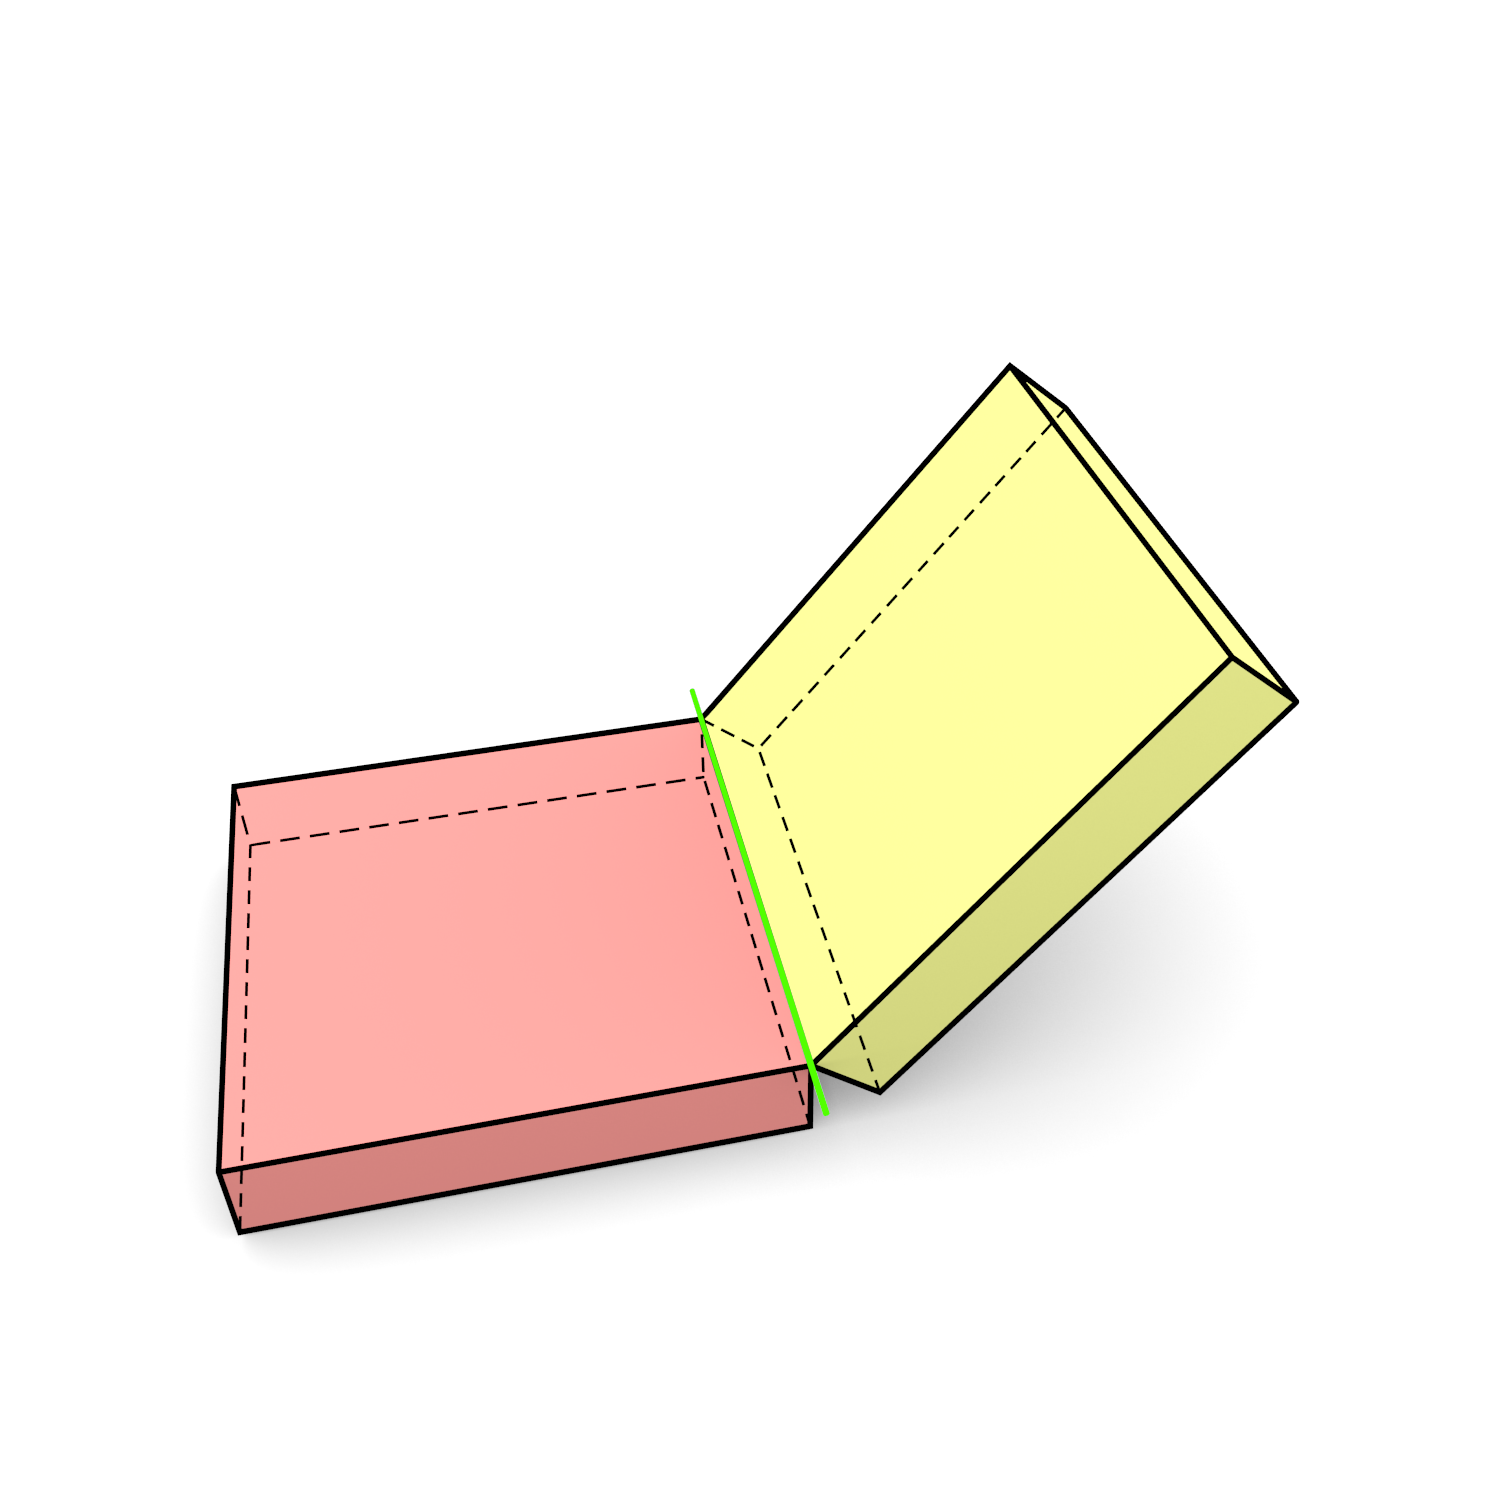
\includegraphics[width=\textwidth]{07-traversing_along_bend_connections_08}
    \caption{The bend axis and the second plate are transformed with the matrix of the first plate.}
    \label{fig:bend-matrix:5}
  \end{subfigure}
  \begin{subfigure}[b]{0.49\textwidth}
    \centering
    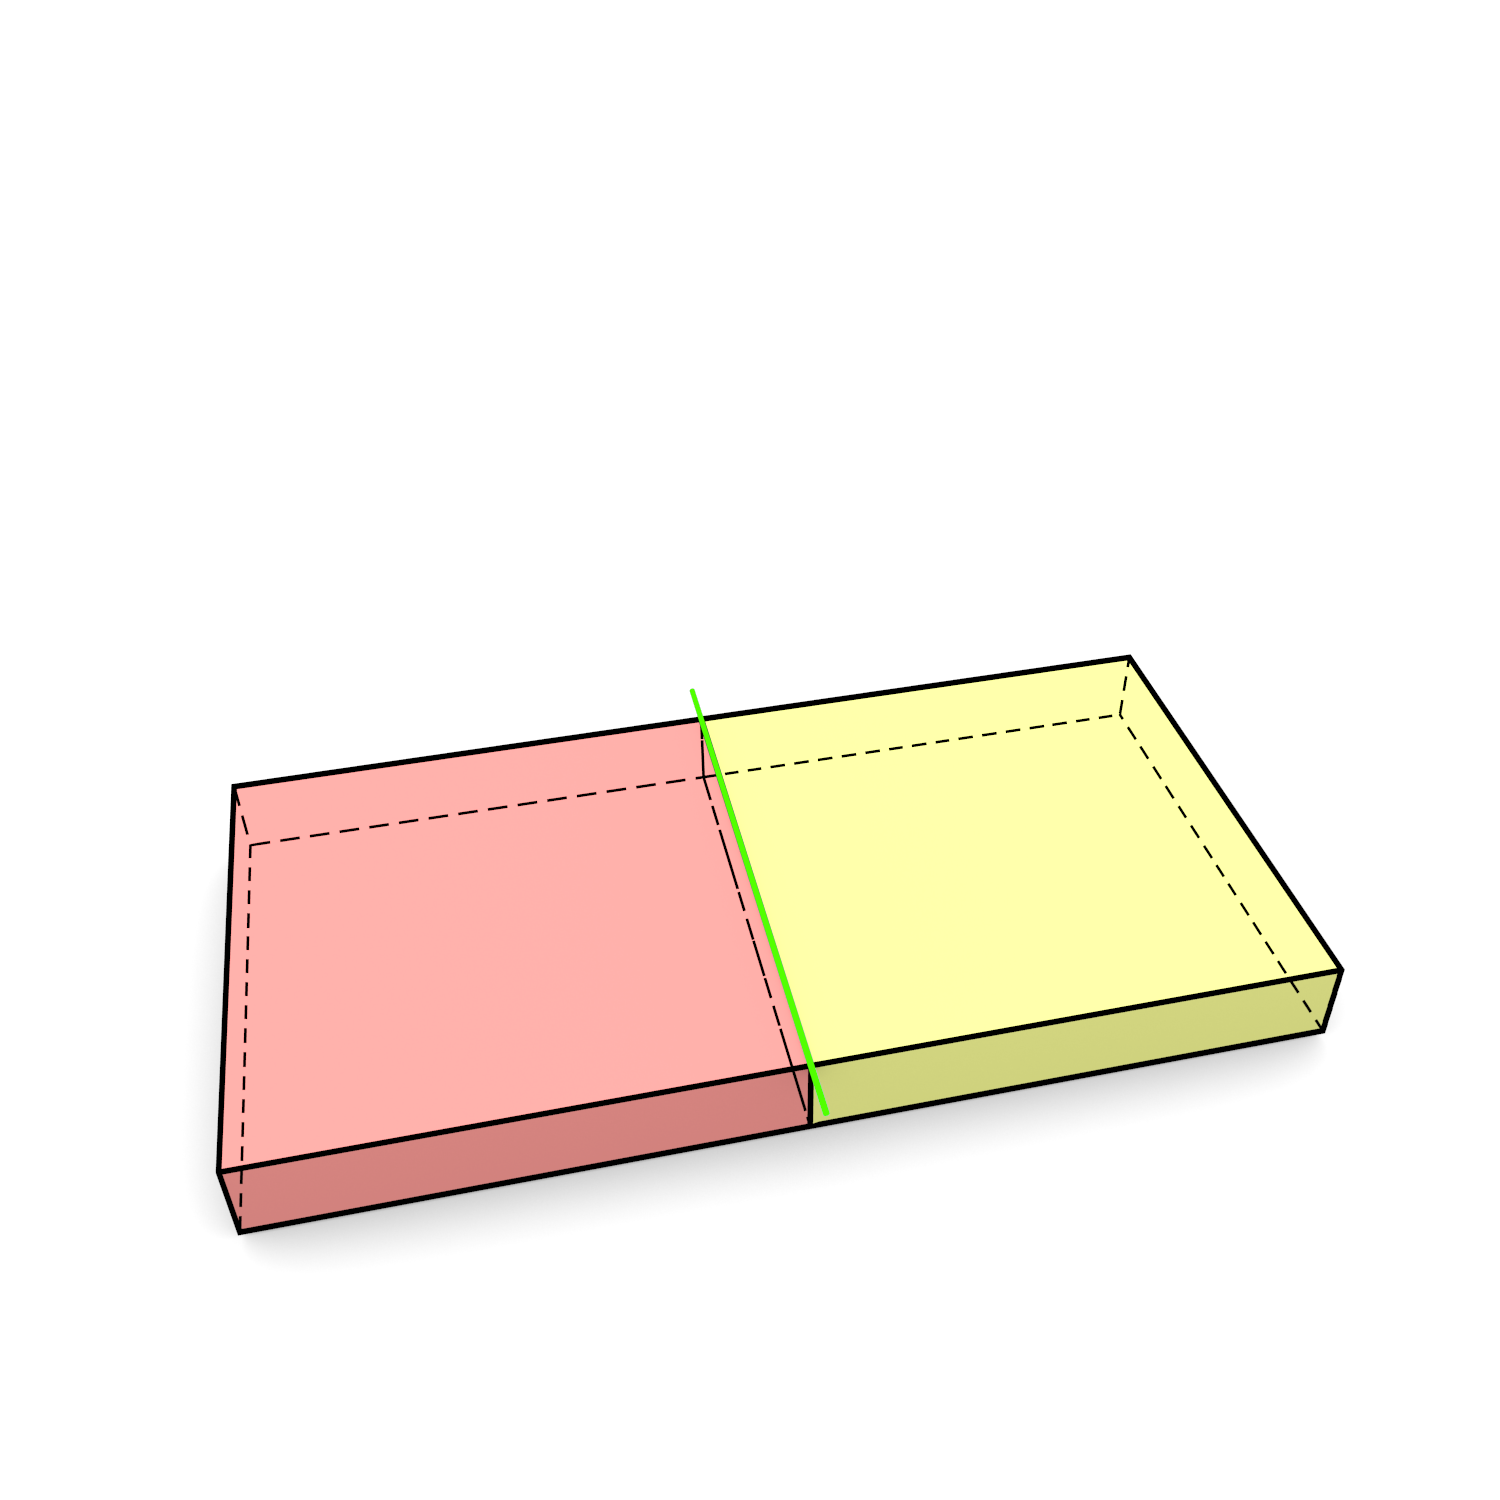
\includegraphics[width=1\textwidth]{07-traversing_along_bend_connections_07}
    \caption{With the new generated transformation matrix the second plate lies in the xy-plane next to the first plate.}
    \label{fig:bend-matrix:6}
  \end{subfigure}
  \caption{Creation steps of the bend matrix.}
  \label{fig:bend-matrix}
\end{figure}

\begin{listing}[ht]
\begin{minted}[
linenos,breaklines
]{coffeescript}
angle = (180 - connection.parameters.angle) * Math.PI / 180
intersectionLine = connection.parameters.intersectionLine
start = intersectionLine.start.clone()

lineDir = plate.shape.normal.clone().cross connection.node.shape.normal
end = start.clone().add lineDir

start = start.applyMatrix4 rotMat
end = end.applyMatrix4 rotMat

axis = start.clone().sub end
axis.normalize()

moveMat1 = new THREE.Matrix4().makeTranslation(
  -start.x,
  -start.y,
  -start.z
)
moveMat2 = new THREE.Matrix4().makeTranslation start.x, start.y, start.z
bendMat = new THREE.Matrix4().makeRotationAxis axis, angle

newRotMat = moveMat2.clone().multiply bendMat
newRotMat = newRotMat.multiply moveMat1
newRotMat = newRotMat.multiply rotMat.clone()
\end{minted}
\caption{Creating the transformation matrix for a plate as part of a bent plate.}
\label{lst:bend-matrix}
\end{listing}

\section{Alternative Solutions}

\subsection{Search for Best Surface Development}

The current implementation does not always find the best solution. While traversing the graph it is possible that there multiple different paths through the graph. This results in unequally good sets of bent plates. For example one way of traversing could create more but smaller bent plates then another.
%One path could be cut by another via an overlap but the better solution would be if the second path along the graph would cut the first.
Because currently only one attempt to traverse the graph is made, the second and probably better option would not be found (see Figure~\ref{fig:better_surface_development}).

We propose following solution to avoid this problem: If a plate which should be added to a bent plate intersects a already added plate, we try removing the present plate and check if adding the new one yields better results.

This will increase the run time and results in better solutions for models where the bendable parts of the \threedmodel{} form a highly connected graph.

\begin{figure}[h]
  \centering
  \begin{subfigure}[b]{0.75\textwidth}
    \centering
    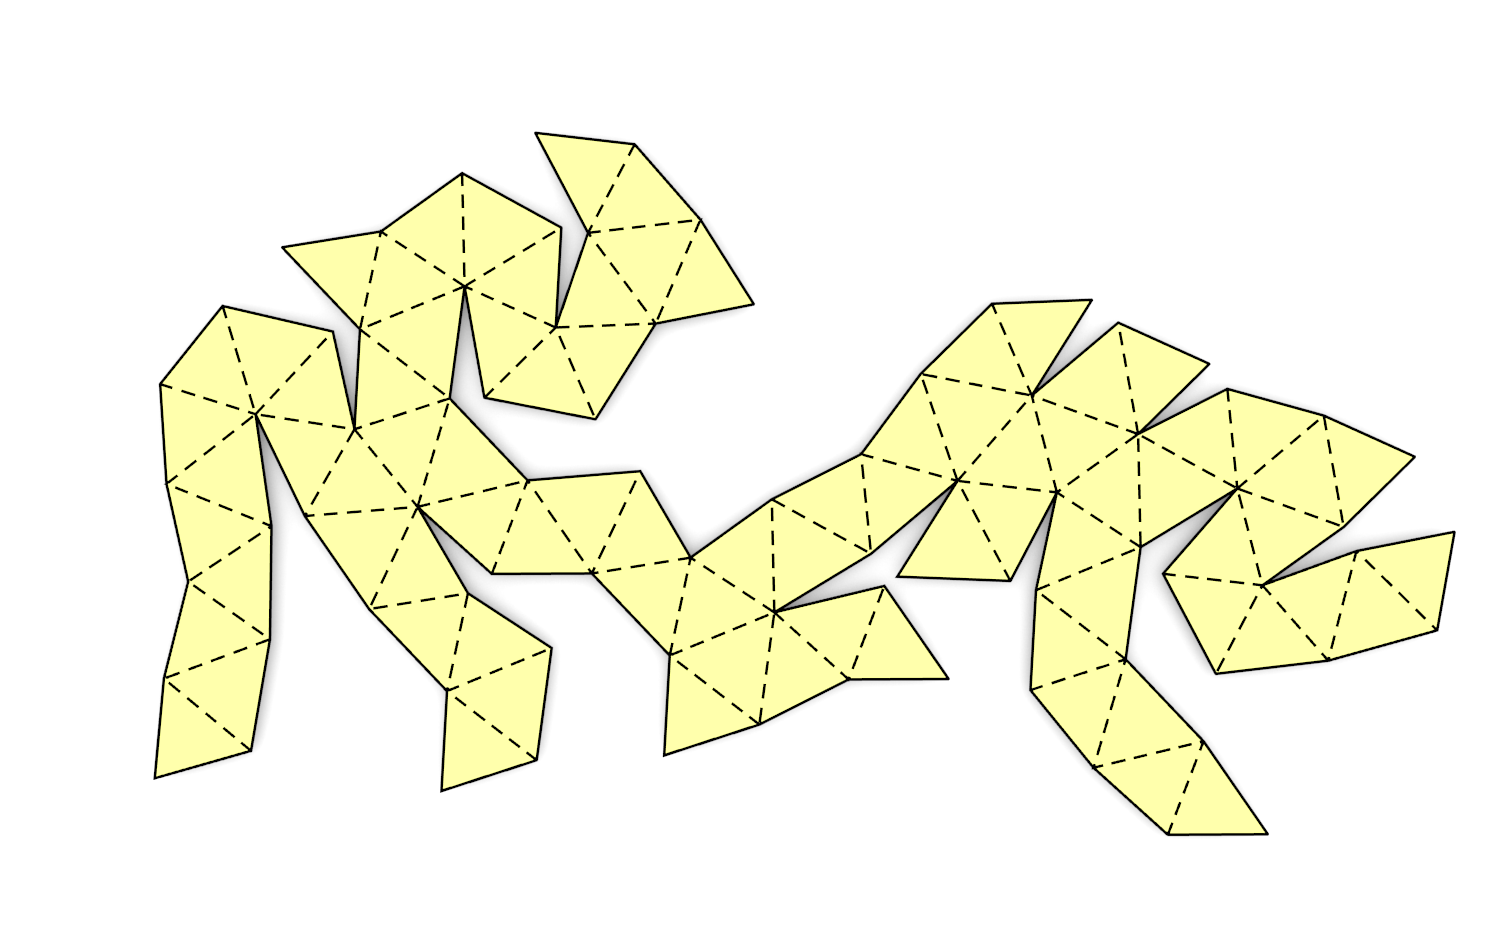
\includegraphics[width=\textwidth]{07-good_surface_development}
    \caption{A surface development of a icosphere without overlaps is possible.}
    \label{fig:overlaps:no-3d}
  \end{subfigure}
  \begin{subfigure}[b]{0.75\textwidth}
    \centering
    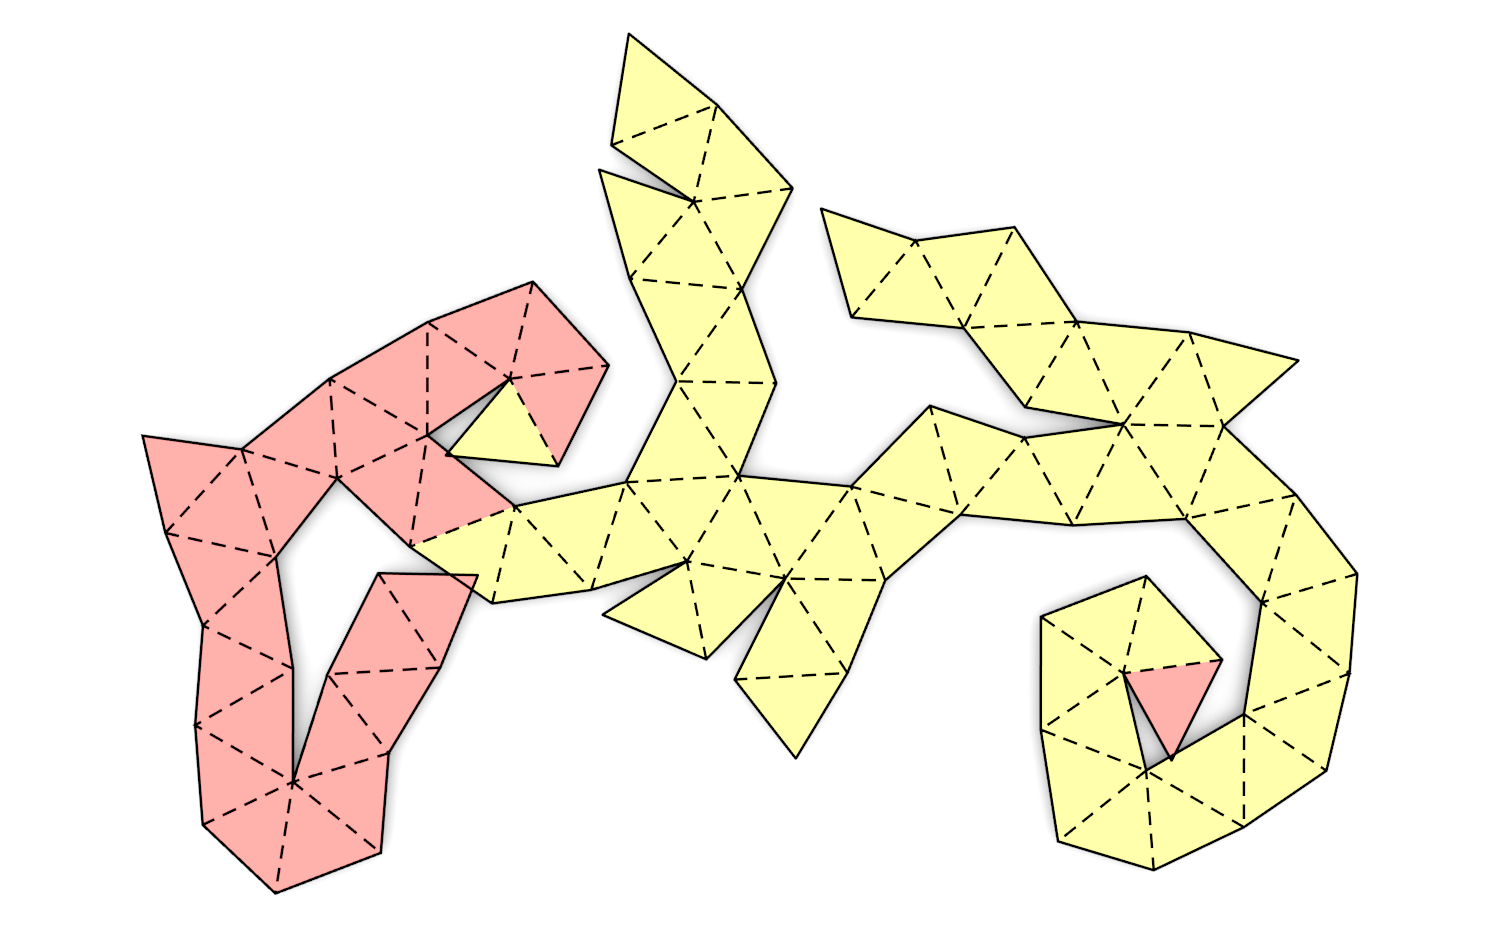
\includegraphics[width=\textwidth]{07-bad_surface_development}
    \caption{If the plate graph is not traversed in a optimal way, overlaps force the algorithm to split the surface into multiple parts.}
    \label{fig:overlapsh:no-2d}
  \end{subfigure}
  \begin{subfigure}[b]{0.75\textwidth}
    \centering
    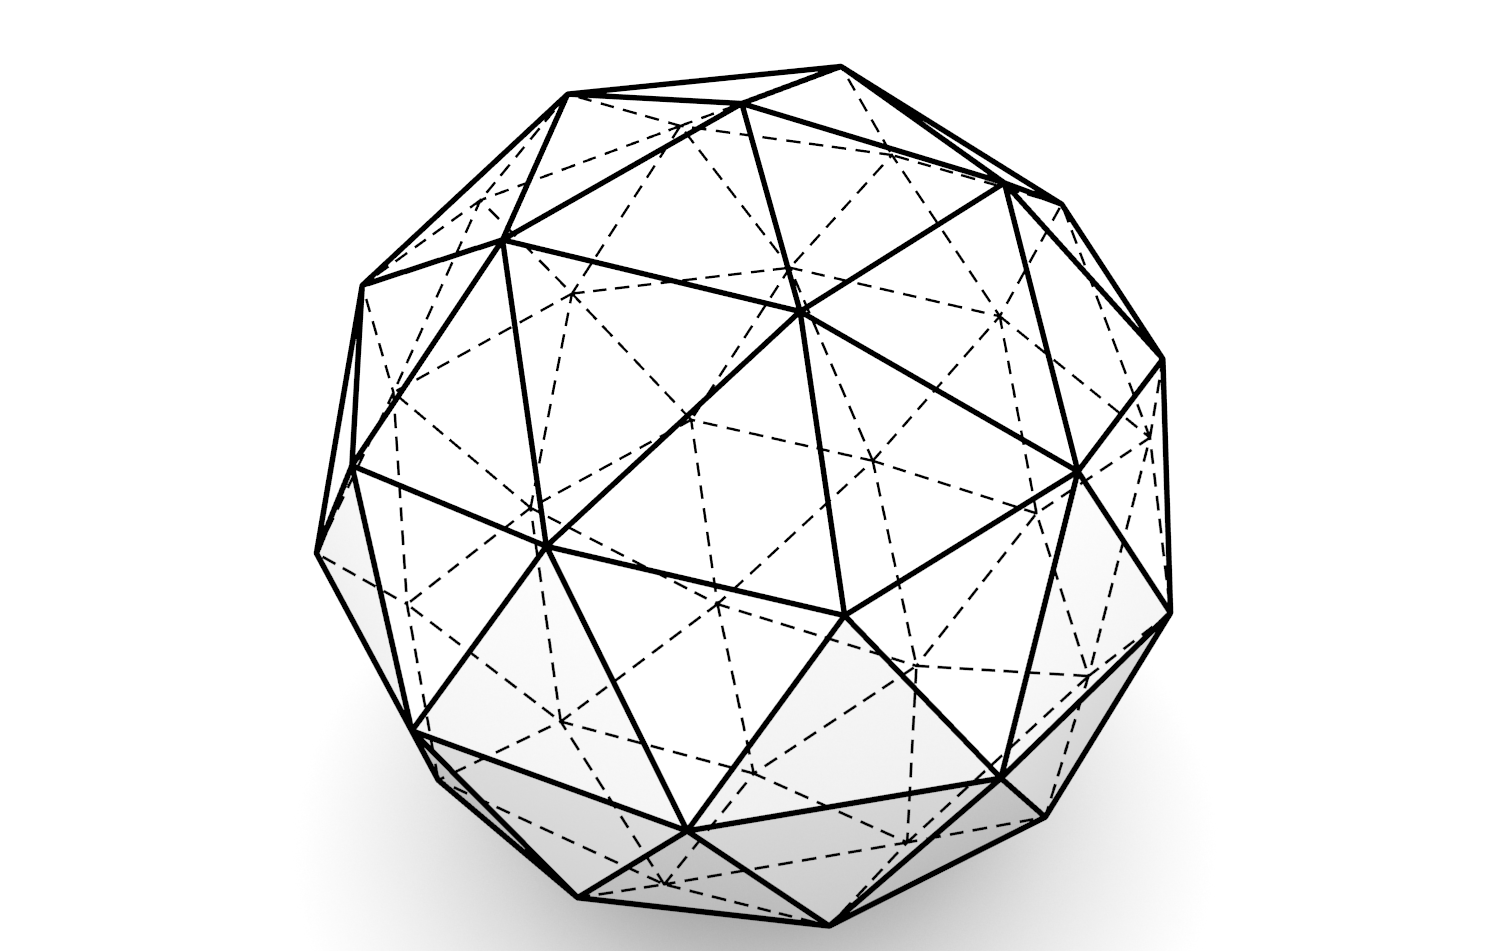
\includegraphics[width=\textwidth]{07-surface_development_model}
    \caption{The model from which the developments where created.}
    \label{fig:overlapsh:no-2d}
  \end{subfigure}
  \caption{The model from which the developments where created.}
  \label{fig:better_surface_development}
\end{figure}

\subsection{Joints at Curved Edges}

Currently the finger joints are generated just based on the plates but not on the bent plates. If multiple small plates which each have to small edges to place finger joints on them are merged into a bent plate, the result would not have finger joints added to it as well.

To avoid this, a new method must be found to generate finger joints at curved edges. Since the edge of the plate that connects to the bent plate  will be curved, the current finger joint algorithm can not be used here. Because adding a plate to the bent plate changes the finger joints, we have to check for overlaps constantly. Thus, the finger joints have to be generate for every attempt to add a new plate.

\subsection{More Bend Line Types}
\label{sec:more_bend_line_types}

 Independently of the used material, a dashed line is added as the bend line. This is good for folding paper. While acrylic can not be bend as easily, we propose engraving a continuous line, which tells the user where to bend the material without weaken the material to much. For wood, on the other side, living hinges should be generated to make the wood bendable at all.

\subsection{Material Dependant Bend Angle}
\label{sec:material_dependant_bend_angle}

Currently the the maximal allowed bending angle is fixed. But because the flexibility of the cut plates differs depending on the used material and thickness, thus should also influence the maximal bend angle. It is also influenced by the bend lines, especially by living hinges, which are designed to change the flexibility (see Section~\sectionref{sec:more_bend_line_types} and \sectionref{sec:living_hinges}).


\end{document}